\documentclass{article}

\usepackage{noweb}
\noweboptions{smallcode,longchunks}
\usepackage[a4paper,margin=1in]{geometry}
\usepackage{caption}
\usepackage{colortbl}
\usepackage[colorlinks=true]{hyperref}
\usepackage{graphicx}

\newcommand{\hi}[1]{\noindent {\bf #1}}     % Define a handy paragraph opener

\def\nwendcode{\endtrivlist \endgroup}      % Remove noweb page break penalty
\let\nwdocspar=\par

\captionsetup{labelfont={bf},textfont={bf,it}}
\setlength{\abovecaptionskip}{1mm}
\setlength{\belowcaptionskip}{1mm}

\title{Jargo Simulation Controller\footnote{
  \url{https://github.com/jargors/Controller}}}
\author{James J. Pan\\
  \small{\href{mailto:pan-j16@mails.tsinghua.edu.cn}{pan-j16@mails.tsinghua.edu.cn}}}

\begin{document}
\maketitle
\pagestyle{noweb}

\tableofcontents

\section{Introduction}
\label{sec:introduction}
The simulation controller is intended to be the sole interface for an
evaluation program to control Jargo's simulation environment. The controller
advances the simulation world time, ``pushes'' server locations and new
requests to the client, perturbs server routes stored in the data layer in
order to mimic traffic and other stochastic vehicle processes, and can be used
to report evaluation metrics to the program.  The simulation controller is
developed using the Noweb\footnote{\url{https://www.cs.tufts.edu/~nr/noweb/}}
literate programming\footnote{\url{http://literateprogramming.com/}} tool.
This file ({\tt{}src/Controller.nw}) is the source for the documentation
({\tt{}doc/Controller.tex}) and the Java code ({\tt{}Controller.java})\footnote{See
the {\tt{}Makefile} for build details.}.

\begin{figure}[h]
\centering
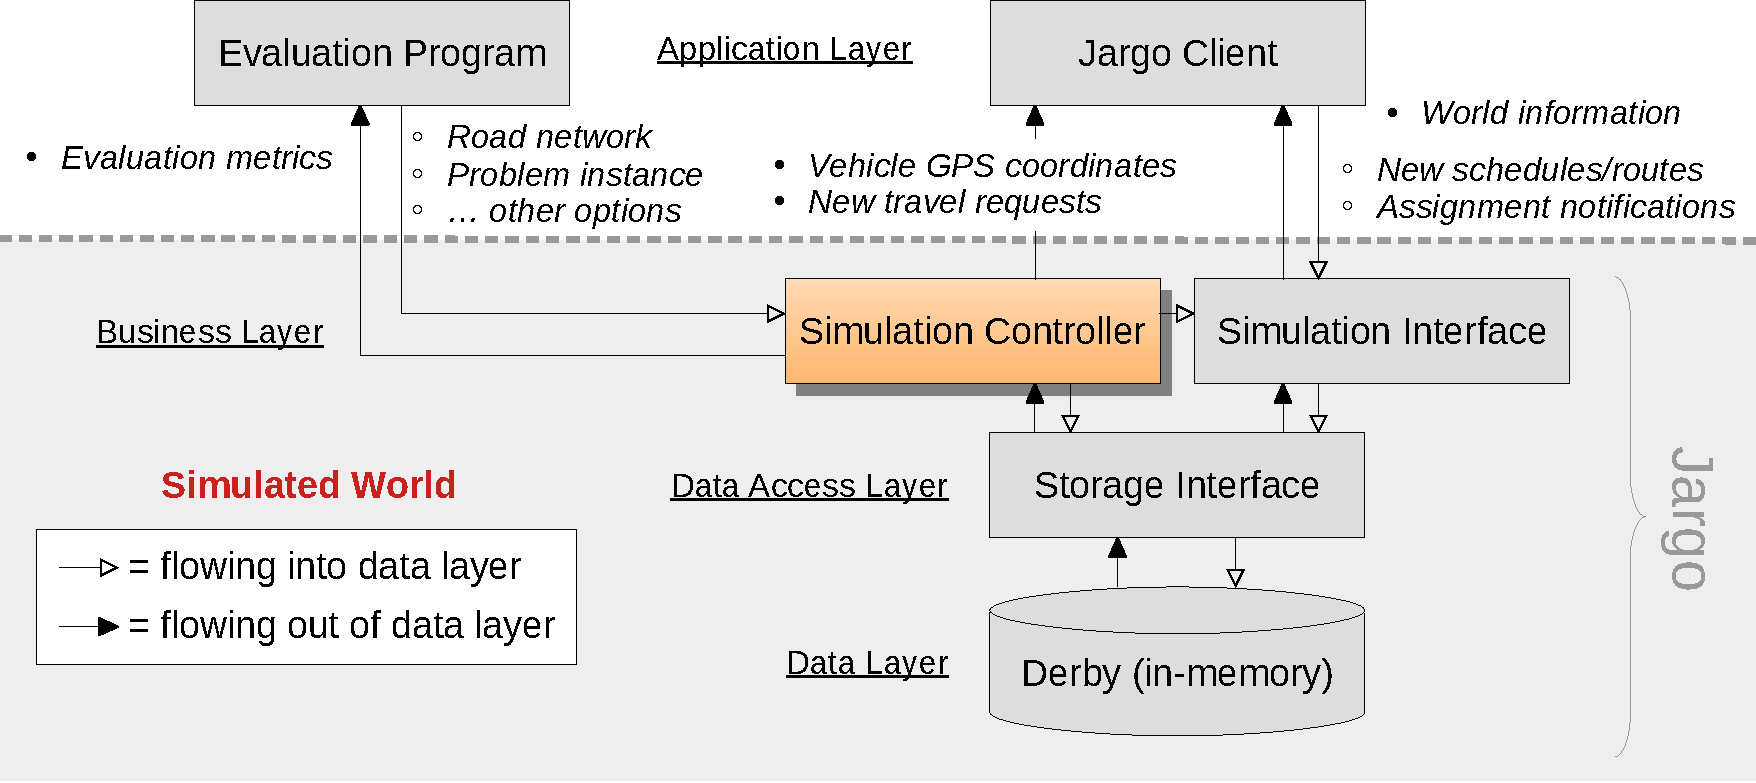
\includegraphics[width=150mm]{src/fig/controller-fig}
\caption{Controller within the Jargo stack.}
\label{fig:controller}
\end{figure}

\section{Implementation Overview}
The code consist of the \emph{preamble} (\S\ref{sec:preamble})
and the \emph{class definition} (\S\ref{sec:class-definition}).
\nwfilename{src/Controller.nw}\nwbegincode{1}\sublabel{NW2ZDXo8-34QoYM-1}\nwmargintag{{\nwtagstyle{}\subpageref{NW2ZDXo8-34QoYM-1}}}\moddef{Controller.java~{\nwtagstyle{}\subpageref{NW2ZDXo8-34QoYM-1}}}\endmoddef\nwnotused{Controller.java}
\LA{}Controller.java preamble~{\nwtagstyle{}\subpageref{NW2ZDXo8-m6OHq-1}}\RA{}
\LA{}\code{}Controller\edoc{} definition~{\nwtagstyle{}\subpageref{NW2ZDXo8-3kvp2C-1}}\RA{}
\nwendcode{}\nwbegindocs{2}\nwdocspar

\subsection{Preamble}
\label{sec:preamble}
The preamble declares the package and imports dependencies.
\nwenddocs{}\nwbegincode{3}\sublabel{NW2ZDXo8-m6OHq-1}\nwmargintag{{\nwtagstyle{}\subpageref{NW2ZDXo8-m6OHq-1}}}\moddef{Controller.java preamble~{\nwtagstyle{}\subpageref{NW2ZDXo8-m6OHq-1}}}\endmoddef\nwalsodefined{\\{NW2ZDXo8-m6OHq-2}\\{NW2ZDXo8-m6OHq-3}\\{NW2ZDXo8-m6OHq-4}\\{NW2ZDXo8-m6OHq-5}\\{NW2ZDXo8-m6OHq-6}\\{NW2ZDXo8-m6OHq-7}}\nwused{\\{NW2ZDXo8-34QoYM-1}}
package com.github.jargors;
\nwendcode{}\nwbegindocs{4}\nwdocspar
We import:
\begin{itemize}
\item all parts of the Jargo stack;
\nwenddocs{}\nwbegincode{5}\sublabel{NW2ZDXo8-m6OHq-2}\nwmargintag{{\nwtagstyle{}\subpageref{NW2ZDXo8-m6OHq-2}}}\moddef{Controller.java preamble~{\nwtagstyle{}\subpageref{NW2ZDXo8-m6OHq-1}}}\plusendmoddef
import com.github.jargors.Storage;
import com.github.jargors.Communicator;
import com.github.jargors.Client;
import com.github.jargors.Tools;
import com.github.jargors.exceptions.DuplicateVertexException;
import com.github.jargors.exceptions.DuplicateEdgeException;
import com.github.jargors.exceptions.DuplicateUserException;
import com.github.jargors.exceptions.EdgeNotFoundException;
import com.github.jargors.exceptions.UserNotFoundException;
import com.github.jargors.exceptions.VertexNotFoundException;
\nwendcode{}\nwbegindocs{6}\item standard utilities for concurrent execution;
\nwenddocs{}\nwbegincode{7}\sublabel{NW2ZDXo8-m6OHq-3}\nwmargintag{{\nwtagstyle{}\subpageref{NW2ZDXo8-m6OHq-3}}}\moddef{Controller.java preamble~{\nwtagstyle{}\subpageref{NW2ZDXo8-m6OHq-1}}}\plusendmoddef
import java.util.concurrent.CompletableFuture;
import java.util.concurrent.Executors;
import java.util.concurrent.ScheduledExecutorService;
import java.util.concurrent.ScheduledFuture;
import java.util.concurrent.TimeUnit;
import java.util.function.Consumer;
\nwendcode{}\nwbegindocs{8}\item standard classes for file operations;
\nwenddocs{}\nwbegincode{9}\sublabel{NW2ZDXo8-m6OHq-4}\nwmargintag{{\nwtagstyle{}\subpageref{NW2ZDXo8-m6OHq-4}}}\moddef{Controller.java preamble~{\nwtagstyle{}\subpageref{NW2ZDXo8-m6OHq-1}}}\plusendmoddef
import java.util.Scanner;
import java.io.File;
import java.io.FileNotFoundException;
\nwendcode{}\nwbegindocs{10}\item date-time class for printing timestamps;
\nwenddocs{}\nwbegincode{11}\sublabel{NW2ZDXo8-m6OHq-5}\nwmargintag{{\nwtagstyle{}\subpageref{NW2ZDXo8-m6OHq-5}}}\moddef{Controller.java preamble~{\nwtagstyle{}\subpageref{NW2ZDXo8-m6OHq-1}}}\plusendmoddef
import java.time.LocalDateTime;
\nwendcode{}\nwbegindocs{12}\item standard map classes for caching various items.
\nwenddocs{}\nwbegincode{13}\sublabel{NW2ZDXo8-m6OHq-6}\nwmargintag{{\nwtagstyle{}\subpageref{NW2ZDXo8-m6OHq-6}}}\moddef{Controller.java preamble~{\nwtagstyle{}\subpageref{NW2ZDXo8-m6OHq-1}}}\plusendmoddef
import java.util.Map;
import java.util.HashMap;
\nwendcode{}\nwbegindocs{14}\nwdocspar
\nwenddocs{}\nwbegincode{15}\sublabel{NW2ZDXo8-m6OHq-7}\nwmargintag{{\nwtagstyle{}\subpageref{NW2ZDXo8-m6OHq-7}}}\moddef{Controller.java preamble~{\nwtagstyle{}\subpageref{NW2ZDXo8-m6OHq-1}}}\plusendmoddef
import java.sql.SQLException;
\nwendcode{}\nwbegindocs{16}\nwdocspar
\end{itemize}

\subsection{Class Definition}
\label{sec:class-definition}
\nwenddocs{}\nwbegincode{17}\sublabel{NW2ZDXo8-3kvp2C-1}\nwmargintag{{\nwtagstyle{}\subpageref{NW2ZDXo8-3kvp2C-1}}}\moddef{\code{}Controller\edoc{} definition~{\nwtagstyle{}\subpageref{NW2ZDXo8-3kvp2C-1}}}\endmoddef\nwused{\\{NW2ZDXo8-34QoYM-1}}
public class Controller \{
  \LA{}\code{}Controller\edoc{} member variables~{\nwtagstyle{}\subpageref{NW2ZDXo8-3yXfwG-1}}\RA{}
  \LA{}\code{}Controller\edoc{} constructor~{\nwtagstyle{}\subpageref{NW2ZDXo8-3AyyZG-1}}\RA{}
  \LA{}\code{}Controller\edoc{} public methods~{\nwtagstyle{}\subpageref{NW2ZDXo8-bF3Hn-1}}\RA{}
\}
\nwendcode{}\nwbegindocs{18}\nwdocspar

\subsection{Member Variables}
Member variables are grouped into \emph{containers}, \emph{settings}, and
\emph{loops}.
\nwenddocs{}\nwbegincode{19}\sublabel{NW2ZDXo8-3yXfwG-1}\nwmargintag{{\nwtagstyle{}\subpageref{NW2ZDXo8-3yXfwG-1}}}\moddef{\code{}Controller\edoc{} member variables~{\nwtagstyle{}\subpageref{NW2ZDXo8-3yXfwG-1}}}\endmoddef\nwused{\\{NW2ZDXo8-3kvp2C-1}}
\LA{}Container objects~{\nwtagstyle{}\subpageref{NW2ZDXo8-OUspt-1}}\RA{}
\LA{}Settings objects~{\nwtagstyle{}\subpageref{NW2ZDXo8-2svhLD-1}}\RA{}
\LA{}Loop objects~{\nwtagstyle{}\subpageref{NW2ZDXo8-2e0Sfa-1}}\RA{}
\nwendcode{}\nwbegindocs{20}\nwdocspar
\hi{Containers.}
\nwenddocs{}\nwbegincode{21}\sublabel{NW2ZDXo8-OUspt-1}\nwmargintag{{\nwtagstyle{}\subpageref{NW2ZDXo8-OUspt-1}}}\moddef{Container objects~{\nwtagstyle{}\subpageref{NW2ZDXo8-OUspt-1}}}\endmoddef\nwused{\\{NW2ZDXo8-3yXfwG-1}}
private Storage storage;
private Communicator communicator;
private Tools tools = new Tools();
private Client client;
private Map<Integer, Boolean> lu_seen = new HashMap<>();
\nwindexdefn{storage}{storage}{NW2ZDXo8-OUspt-1}\nwindexdefn{communicator}{communicator}{NW2ZDXo8-OUspt-1}\nwindexdefn{tools}{tools}{NW2ZDXo8-OUspt-1}\nwindexdefn{client}{client}{NW2ZDXo8-OUspt-1}\nwindexdefn{lu{\char95}seen}{lu:unseen}{NW2ZDXo8-OUspt-1}\eatline
\nwidentdefs{\\{{client}{client}}\\{{communicator}{communicator}}\\{{lu{\char95}seen}{lu:unseen}}\\{{storage}{storage}}\\{{tools}{tools}}}\nwendcode{}\nwbegindocs{22}\nwdocspar
\hi{Settings.} Settings objects configure various aspects of the simulation.
These settings should mostly be set by the evaluation program by using the public
setters.

Ultimately we want everything in the database to be an integer so we don't have
to fiddle around with data types when we do reads and writes. We use {\tt{}\protect\nwindexuse{CSHIFT}{CSHIFT}{NW2ZDXo8-2svhLD-1}CSHIFT}
to shift the decimal places of latitude and longitude coordinates left and
right by multiplication or division\footnote{Beware, if {\tt{}\protect\nwindexuse{CSHIFT}{CSHIFT}{NW2ZDXo8-2svhLD-1}CSHIFT} is changed
here, it should also be changed in Tools.}.
\nwenddocs{}\nwbegincode{23}\sublabel{NW2ZDXo8-2svhLD-1}\nwmargintag{{\nwtagstyle{}\subpageref{NW2ZDXo8-2svhLD-1}}}\moddef{Settings objects~{\nwtagstyle{}\subpageref{NW2ZDXo8-2svhLD-1}}}\endmoddef\nwused{\\{NW2ZDXo8-3yXfwG-1}}
private final double CSHIFT = 10000000.0;
private static int world_time = 0;
private int initial_world_time = 0;
private int final_world_time = 86400;
private int engine_update_period = 10;
private int loop_delay = 0;
// private int deviation_rate = 0.02;
// private int breakdown_rate = 0.005;
\nwindexdefn{CSHIFT}{CSHIFT}{NW2ZDXo8-2svhLD-1}\nwindexdefn{world{\char95}time}{world:untime}{NW2ZDXo8-2svhLD-1}\nwindexdefn{initial{\char95}world{\char95}time}{initial:unworld:untime}{NW2ZDXo8-2svhLD-1}\nwindexdefn{final{\char95}world{\char95}time}{final:unworld:untime}{NW2ZDXo8-2svhLD-1}\nwindexdefn{engine{\char95}update{\char95}period}{engine:unupdate:unperiod}{NW2ZDXo8-2svhLD-1}\nwindexdefn{loop{\char95}delay}{loop:undelay}{NW2ZDXo8-2svhLD-1}\eatline
\nwidentdefs{\\{{CSHIFT}{CSHIFT}}\\{{engine{\char95}update{\char95}period}{engine:unupdate:unperiod}}\\{{final{\char95}world{\char95}time}{final:unworld:untime}}\\{{initial{\char95}world{\char95}time}{initial:unworld:untime}}\\{{loop{\char95}delay}{loop:undelay}}\\{{world{\char95}time}{world:untime}}}\nwendcode{}\nwbegindocs{24}\nwdocspar
\hi{Loops.} Jargo's simulation environment comprises four ``loops'', defined
here, running in parallel. They are executed using Java's
{\tt{}ScheduledExecutorService} to control timing.
\nwenddocs{}\nwbegincode{25}\sublabel{NW2ZDXo8-2e0Sfa-1}\nwmargintag{{\nwtagstyle{}\subpageref{NW2ZDXo8-2e0Sfa-1}}}\moddef{Loop objects~{\nwtagstyle{}\subpageref{NW2ZDXo8-2e0Sfa-1}}}\endmoddef\nwused{\\{NW2ZDXo8-3yXfwG-1}}
\LA{}Definition of clock loop~{\nwtagstyle{}\subpageref{NW2ZDXo8-2lFPcZ-1}}\RA{}
\LA{}Definition of engine loop~{\nwtagstyle{}\subpageref{NW2ZDXo8-3rcRXt-1}}\RA{}
\LA{}Definition of request collection loop~{\nwtagstyle{}\subpageref{NW2ZDXo8-10L3rI-1}}\RA{}
\LA{}Definition of request handling loop~{\nwtagstyle{}\subpageref{NW2ZDXo8-183plv-1}}\RA{}
\LA{}Definition of server collection loop~{\nwtagstyle{}\subpageref{NW2ZDXo8-1I3SnY-1}}\RA{}
\nwendcode{}\nwbegindocs{26}\nwdocspar

\subsubsection{Clock Loop}
This loop advances the simulation world time.
\nwenddocs{}\nwbegincode{27}\sublabel{NW2ZDXo8-2lFPcZ-1}\nwmargintag{{\nwtagstyle{}\subpageref{NW2ZDXo8-2lFPcZ-1}}}\moddef{Definition of clock loop~{\nwtagstyle{}\subpageref{NW2ZDXo8-2lFPcZ-1}}}\endmoddef\nwused{\\{NW2ZDXo8-2e0Sfa-1}}
private Runnable ClockLoop = () -> \{
  communicator.setSimulationWorldTime(++world_time);
  Tools.Print((world_time % 2 == 0 ? "*ping*" : "*pong*"));
\};
\nwindexdefn{ClockLoop}{ClockLoop}{NW2ZDXo8-2lFPcZ-1}\eatline
\nwidentdefs{\\{{ClockLoop}{ClockLoop}}}\nwidentuses{\\{{communicator}{communicator}}\\{{world{\char95}time}{world:untime}}}\nwindexuse{communicator}{communicator}{NW2ZDXo8-2lFPcZ-1}\nwindexuse{world{\char95}time}{world:untime}{NW2ZDXo8-2lFPcZ-1}\nwendcode{}\nwbegindocs{28}\nwdocspar
\subsubsection{Engine Loop}
\nwenddocs{}\nwbegincode{29}\sublabel{NW2ZDXo8-3rcRXt-1}\nwmargintag{{\nwtagstyle{}\subpageref{NW2ZDXo8-3rcRXt-1}}}\moddef{Definition of engine loop~{\nwtagstyle{}\subpageref{NW2ZDXo8-3rcRXt-1}}}\endmoddef\nwused{\\{NW2ZDXo8-2e0Sfa-1}}
private Runnable EngineLoop = () -> \{ \};
\nwindexdefn{EngineLoop}{EngineLoop}{NW2ZDXo8-3rcRXt-1}\eatline
\nwidentdefs{\\{{EngineLoop}{EngineLoop}}}\nwendcode{}\nwbegindocs{30}\nwdocspar
\subsubsection{Request Collection Loop}
\nwenddocs{}\nwbegincode{31}\sublabel{NW2ZDXo8-10L3rI-1}\nwmargintag{{\nwtagstyle{}\subpageref{NW2ZDXo8-10L3rI-1}}}\moddef{Definition of request collection loop~{\nwtagstyle{}\subpageref{NW2ZDXo8-10L3rI-1}}}\endmoddef\nwused{\\{NW2ZDXo8-2e0Sfa-1}}
private Runnable RequestCollectionLoop = () -> \{
  long A0 = System.currentTimeMillis();
  final int t0 = world_time;
  try \{
    int[] output = storage.DBQueryQueuedRequests(world_time);
    for (int i = 0; i < (output.length - 6); i += 7) \{
      if (!lu_seen.containsKey(output[i]) || lu_seen.get(output[i]) == false) \{
        client.collectRequest(new int[] \{
          output[(i + 0)],
          output[(i + 1)],
          output[(i + 2)],
          output[(i + 3)],
          output[(i + 4)],
          output[(i + 5)],
          output[(i + 6)] \});
        lu_seen.put(output[i], true);
      \}
    \}
  \} catch (SQLException e) \{
    System.err.println("Encountered fatal error");
    Tools.PrintSQLException(e);
    System.exit(1);
  \}
  final int t1 = world_time;
  long A1 = System.currentTimeMillis();
  Tools.Print("Time RCL: "+(A1 - A0)+" ms");
\};
\nwindexdefn{RequestCollectionLoop}{RequestCollectionLoop}{NW2ZDXo8-10L3rI-1}\eatline
\nwidentdefs{\\{{RequestCollectionLoop}{RequestCollectionLoop}}}\nwidentuses{\\{{client}{client}}\\{{lu{\char95}seen}{lu:unseen}}\\{{storage}{storage}}\\{{world{\char95}time}{world:untime}}}\nwindexuse{client}{client}{NW2ZDXo8-10L3rI-1}\nwindexuse{lu{\char95}seen}{lu:unseen}{NW2ZDXo8-10L3rI-1}\nwindexuse{storage}{storage}{NW2ZDXo8-10L3rI-1}\nwindexuse{world{\char95}time}{world:untime}{NW2ZDXo8-10L3rI-1}\nwendcode{}\nwbegindocs{32}\nwdocspar
\subsubsection{Request Handling Loop}
\nwenddocs{}\nwbegincode{33}\sublabel{NW2ZDXo8-183plv-1}\nwmargintag{{\nwtagstyle{}\subpageref{NW2ZDXo8-183plv-1}}}\moddef{Definition of request handling loop~{\nwtagstyle{}\subpageref{NW2ZDXo8-183plv-1}}}\endmoddef\nwused{\\{NW2ZDXo8-2e0Sfa-1}}
private Runnable RequestHandlingLoop = () -> \{
  long A0 = System.currentTimeMillis();
  try \{
    client.notifyNew();
  \} catch (RuntimeException e) \{
    System.out.println("client.notifyNew() exception: "+e.toString());
  \}
  long A1 = System.currentTimeMillis();
  Tools.Print("Time RHL: "+(A1 - A0)+" ms");
\};
\nwindexdefn{RequestHandlingLoop}{RequestHandlingLoop}{NW2ZDXo8-183plv-1}\eatline
\nwidentdefs{\\{{RequestHandlingLoop}{RequestHandlingLoop}}}\nwidentuses{\\{{client}{client}}}\nwindexuse{client}{client}{NW2ZDXo8-183plv-1}\nwendcode{}\nwbegindocs{34}\nwdocspar
\subsubsection{Server Loop}
This loop ``pushes'' server locations to the client.
Option A. Cache the routes here, then update the cache when the routes change.
Option B. Change the query to use one query to get active vehicles, then
  a second query to get position from table W for each active vehicle, instead
  of using join.
\nwenddocs{}\nwbegincode{35}\sublabel{NW2ZDXo8-1I3SnY-1}\nwmargintag{{\nwtagstyle{}\subpageref{NW2ZDXo8-1I3SnY-1}}}\moddef{Definition of server collection loop~{\nwtagstyle{}\subpageref{NW2ZDXo8-1I3SnY-1}}}\endmoddef\nwused{\\{NW2ZDXo8-2e0Sfa-1}}
private Runnable ServerLoop = () -> \{
  long A0 = System.currentTimeMillis();
  try \{
    int[] output = storage.DBQueryServerLocationsActive(world_time);
    client.collectServerLocations(output);
  \} catch (SQLException e) \{
    System.err.println("Encountered fatal error");
    Tools.PrintSQLException(e);
    System.exit(1);
  \}
  long A1 = System.currentTimeMillis();
  Tools.Print("Time SL: "+(A1 - A0)+" ms");
\};
\nwindexdefn{ServerLoop}{ServerLoop}{NW2ZDXo8-1I3SnY-1}\eatline
\nwidentdefs{\\{{ServerLoop}{ServerLoop}}}\nwidentuses{\\{{client}{client}}\\{{storage}{storage}}\\{{world{\char95}time}{world:untime}}}\nwindexuse{client}{client}{NW2ZDXo8-1I3SnY-1}\nwindexuse{storage}{storage}{NW2ZDXo8-1I3SnY-1}\nwindexuse{world{\char95}time}{world:untime}{NW2ZDXo8-1I3SnY-1}\nwendcode{}\nwbegindocs{36}\nwdocspar
\subsection{Constructor}
\nwenddocs{}\nwbegincode{37}\sublabel{NW2ZDXo8-3AyyZG-1}\nwmargintag{{\nwtagstyle{}\subpageref{NW2ZDXo8-3AyyZG-1}}}\moddef{\code{}Controller\edoc{} constructor~{\nwtagstyle{}\subpageref{NW2ZDXo8-3AyyZG-1}}}\endmoddef\nwused{\\{NW2ZDXo8-3kvp2C-1}}
public Controller() \{
  storage = new Storage();
  communicator = new Communicator();
  communicator.setStorage(storage);
  communicator.setController(this);
\}
\nwidentuses{\\{{communicator}{communicator}}\\{{storage}{storage}}}\nwindexuse{communicator}{communicator}{NW2ZDXo8-3AyyZG-1}\nwindexuse{storage}{storage}{NW2ZDXo8-3AyyZG-1}\nwendcode{}\nwbegindocs{38}\nwdocspar

\section{Public Methods}
\label{sec:public-methods}
\hi{General methods.}
\nwenddocs{}\nwbegincode{39}\sublabel{NW2ZDXo8-bF3Hn-1}\nwmargintag{{\nwtagstyle{}\subpageref{NW2ZDXo8-bF3Hn-1}}}\moddef{\code{}Controller\edoc{} public methods~{\nwtagstyle{}\subpageref{NW2ZDXo8-bF3Hn-1}}}\endmoddef\nwalsodefined{\\{NW2ZDXo8-bF3Hn-2}\\{NW2ZDXo8-bF3Hn-3}}\nwused{\\{NW2ZDXo8-3kvp2C-1}}
\LA{}Initialize new empty database~{\nwtagstyle{}\subpageref{NW2ZDXo8-2CVxut-1}}\RA{}
\LA{}Close database~{\nwtagstyle{}\subpageref{NW2ZDXo8-3A3oOU-1}}\RA{}
\LA{}Set client debug~{\nwtagstyle{}\subpageref{NW2ZDXo8-2O3rxF-1}}\RA{}
\LA{}Set communicator debug~{\nwtagstyle{}\subpageref{NW2ZDXo8-272uK2-1}}\RA{}
\LA{}Set client~{\nwtagstyle{}\subpageref{NW2ZDXo8-3HnCZ3-1}}\RA{}
\LA{}Set initial world time~{\nwtagstyle{}\subpageref{NW2ZDXo8-3BZAWj-1}}\RA{}
\LA{}Set final world time~{\nwtagstyle{}\subpageref{NW2ZDXo8-2PAB4K-1}}\RA{}
\LA{}Get world time~{\nwtagstyle{}\subpageref{NW2ZDXo8-3X8zhz-1}}\RA{}
\LA{}Return request to queue~{\nwtagstyle{}\subpageref{NW2ZDXo8-3SURrj-1}}\RA{}
\LA{}Save backup~{\nwtagstyle{}\subpageref{NW2ZDXo8-2OKmqF-1}}\RA{}
\LA{}Load backup~{\nwtagstyle{}\subpageref{NW2ZDXo8-b3Hn1-1}}\RA{}
\LA{}Load data model~{\nwtagstyle{}\subpageref{NW2ZDXo8-4P4YpK-1}}\RA{}
\LA{}Load road network~{\nwtagstyle{}\subpageref{NW2ZDXo8-1JUvcB-1}}\RA{}
\LA{}Load problem~{\nwtagstyle{}\subpageref{NW2ZDXo8-2rtVpi-1}}\RA{}
\LA{}Load GTree~{\nwtagstyle{}\subpageref{NW2ZDXo8-b7Jka-1}}\RA{}
\LA{}Start dynamic simulation~{\nwtagstyle{}\subpageref{NW2ZDXo8-43uvLJ-1}}\RA{}
\LA{}Start static simulation~{\nwtagstyle{}\subpageref{NW2ZDXo8-1n2dd-1}}\RA{}
\nwendcode{}\nwbegindocs{40}\nwdocspar
\hi{Read methods.}
\nwenddocs{}\nwbegincode{41}\sublabel{NW2ZDXo8-bF3Hn-2}\nwmargintag{{\nwtagstyle{}\subpageref{NW2ZDXo8-bF3Hn-2}}}\moddef{\code{}Controller\edoc{} public methods~{\nwtagstyle{}\subpageref{NW2ZDXo8-bF3Hn-1}}}\plusendmoddef
\LA{}Query custom statement~{\nwtagstyle{}\subpageref{NW2ZDXo8-2FtqIZ-1}}\RA{}
\LA{}Query all vertices~{\nwtagstyle{}\subpageref{NW2ZDXo8-1r5OnM-1}}\RA{}
\LA{}Query all edges~{\nwtagstyle{}\subpageref{NW2ZDXo8-4ILREc-1}}\RA{}
\LA{}Query vertex~{\nwtagstyle{}\subpageref{NW2ZDXo8-4IfXsG-1}}\RA{}
\LA{}Query edge~{\nwtagstyle{}\subpageref{NW2ZDXo8-1E2aru-1}}\RA{}
\LA{}Query ridesharing user~{\nwtagstyle{}\subpageref{NW2ZDXo8-3isdeu-1}}\RA{}
\LA{}Query queued requests~{\nwtagstyle{}\subpageref{NW2ZDXo8-3AGrxZ-1}}\RA{}
\LA{}Query routes~{\nwtagstyle{}\subpageref{NW2ZDXo8-1AprqI-1}}\RA{}
\LA{}Query schedules~{\nwtagstyle{}\subpageref{NW2ZDXo8-3yA8FQ-1}}\RA{}
\LA{}Query various metrics~{\nwtagstyle{}\subpageref{NW2ZDXo8-1Ang64-1}}\RA{}
\nwendcode{}\nwbegindocs{42}\nwdocspar
\hi{Write methods.}
\nwenddocs{}\nwbegincode{43}\sublabel{NW2ZDXo8-bF3Hn-3}\nwmargintag{{\nwtagstyle{}\subpageref{NW2ZDXo8-bF3Hn-3}}}\moddef{\code{}Controller\edoc{} public methods~{\nwtagstyle{}\subpageref{NW2ZDXo8-bF3Hn-1}}}\plusendmoddef
\LA{}Add new server~{\nwtagstyle{}\subpageref{NW2ZDXo8-IYVQQ-1}}\RA{}
\LA{}Add new request~{\nwtagstyle{}\subpageref{NW2ZDXo8-4ISWm4-1}}\RA{}
\nwendcode{}\nwbegindocs{44}\nwdocspar

\subsection{General methods}

\subsubsection{{\tt{}\protect\nosublabel{NW2ZDXo8-bF3Hn-3-u2}\protect\nwindexuse{createNewInstance}{createNewInstance}{NW2ZDXo8-2CVxut-1}createNewInstance}(0)}
\nwenddocs{}\nwbegincode{45}\sublabel{NW2ZDXo8-2CVxut-1}\nwmargintag{{\nwtagstyle{}\subpageref{NW2ZDXo8-2CVxut-1}}}\moddef{Initialize new empty database~{\nwtagstyle{}\subpageref{NW2ZDXo8-2CVxut-1}}}\endmoddef\nwused{\\{NW2ZDXo8-bF3Hn-1}}
public void createNewInstance() \{
  try \{
    storage.DBCreateNewInstance();
  \} catch (SQLException e) \{
    System.err.println("Encountered fatal error");
    Tools.PrintSQLException(e);
    System.exit(1);
  \}
\}
\nwindexdefn{createNewInstance}{createNewInstance}{NW2ZDXo8-2CVxut-1}\eatline
\nwidentdefs{\\{{createNewInstance}{createNewInstance}}}\nwidentuses{\\{{storage}{storage}}}\nwindexuse{storage}{storage}{NW2ZDXo8-2CVxut-1}\nwendcode{}\nwbegindocs{46}\nwdocspar
\subsubsection{{\tt{}\protect\nwindexuse{closeInstance}{closeInstance}{NW2ZDXo8-3A3oOU-1}closeInstance}(0)}
\nwenddocs{}\nwbegincode{47}\sublabel{NW2ZDXo8-3A3oOU-1}\nwmargintag{{\nwtagstyle{}\subpageref{NW2ZDXo8-3A3oOU-1}}}\moddef{Close database~{\nwtagstyle{}\subpageref{NW2ZDXo8-3A3oOU-1}}}\endmoddef\nwused{\\{NW2ZDXo8-bF3Hn-1}}
public void closeInstance() \{
  try \{
    storage.DBCloseInstance();
  \} catch (SQLException e) \{
    System.err.println("Encountered fatal error");
    Tools.PrintSQLException(e);
    System.exit(1);
  \}
\}
\nwindexdefn{closeInstance}{closeInstance}{NW2ZDXo8-3A3oOU-1}\eatline
\nwidentdefs{\\{{closeInstance}{closeInstance}}}\nwidentuses{\\{{storage}{storage}}}\nwindexuse{storage}{storage}{NW2ZDXo8-3A3oOU-1}\nwendcode{}\nwbegindocs{48}\nwdocspar
\subsubsection{{\tt{}\protect\nwindexuse{setDebugClient}{setDebugClient}{NW2ZDXo8-2O3rxF-1}setDebugClient}(1)}
\nwenddocs{}\nwbegincode{49}\sublabel{NW2ZDXo8-2O3rxF-1}\nwmargintag{{\nwtagstyle{}\subpageref{NW2ZDXo8-2O3rxF-1}}}\moddef{Set client debug~{\nwtagstyle{}\subpageref{NW2ZDXo8-2O3rxF-1}}}\endmoddef\nwused{\\{NW2ZDXo8-bF3Hn-1}}
public void setDebugClient(boolean flag) \{
  client.setDebug(flag);
\}
\nwindexdefn{setDebugClient}{setDebugClient}{NW2ZDXo8-2O3rxF-1}\eatline
\nwidentdefs{\\{{setDebugClient}{setDebugClient}}}\nwidentuses{\\{{client}{client}}}\nwindexuse{client}{client}{NW2ZDXo8-2O3rxF-1}\nwendcode{}\nwbegindocs{50}\nwdocspar
\subsubsection{{\tt{}\protect\nwindexuse{setDebugCommunicator}{setDebugCommunicator}{NW2ZDXo8-272uK2-1}setDebugCommunicator}(1)}
\nwenddocs{}\nwbegincode{51}\sublabel{NW2ZDXo8-272uK2-1}\nwmargintag{{\nwtagstyle{}\subpageref{NW2ZDXo8-272uK2-1}}}\moddef{Set communicator debug~{\nwtagstyle{}\subpageref{NW2ZDXo8-272uK2-1}}}\endmoddef\nwused{\\{NW2ZDXo8-bF3Hn-1}}
public void setDebugCommunicator(boolean flag) \{
  communicator.setDebug(flag);
\}
\nwindexdefn{setDebugCommunicator}{setDebugCommunicator}{NW2ZDXo8-272uK2-1}\eatline
\nwidentdefs{\\{{setDebugCommunicator}{setDebugCommunicator}}}\nwidentuses{\\{{communicator}{communicator}}}\nwindexuse{communicator}{communicator}{NW2ZDXo8-272uK2-1}\nwendcode{}\nwbegindocs{52}\nwdocspar
\subsubsection{{\tt{}\protect\nwindexuse{setClient}{setClient}{NW2ZDXo8-3HnCZ3-1}setClient}(1)}
\nwenddocs{}\nwbegincode{53}\sublabel{NW2ZDXo8-3HnCZ3-1}\nwmargintag{{\nwtagstyle{}\subpageref{NW2ZDXo8-3HnCZ3-1}}}\moddef{Set client~{\nwtagstyle{}\subpageref{NW2ZDXo8-3HnCZ3-1}}}\endmoddef\nwused{\\{NW2ZDXo8-bF3Hn-1}}
public void setClient(Client target) \{
  client = target;
  client.setCommunicator(communicator);
\}
\nwindexdefn{setClient}{setClient}{NW2ZDXo8-3HnCZ3-1}\eatline
\nwidentdefs{\\{{setClient}{setClient}}}\nwidentuses{\\{{client}{client}}\\{{communicator}{communicator}}}\nwindexuse{client}{client}{NW2ZDXo8-3HnCZ3-1}\nwindexuse{communicator}{communicator}{NW2ZDXo8-3HnCZ3-1}\nwendcode{}\nwbegindocs{54}\nwdocspar
\subsubsection{{\tt{}\protect\nwindexuse{setInitialWorldTime}{setInitialWorldTime}{NW2ZDXo8-3BZAWj-1}setInitialWorldTime(1)}}
\nwenddocs{}\nwbegincode{55}\sublabel{NW2ZDXo8-3BZAWj-1}\nwmargintag{{\nwtagstyle{}\subpageref{NW2ZDXo8-3BZAWj-1}}}\moddef{Set initial world time~{\nwtagstyle{}\subpageref{NW2ZDXo8-3BZAWj-1}}}\endmoddef\nwused{\\{NW2ZDXo8-bF3Hn-1}}
public void setInitialWorldTime(int t) \{
  initial_world_time = t;
\}
\nwindexdefn{setInitialWorldTime}{setInitialWorldTime}{NW2ZDXo8-3BZAWj-1}\eatline
\nwidentdefs{\\{{setInitialWorldTime}{setInitialWorldTime}}}\nwidentuses{\\{{initial{\char95}world{\char95}time}{initial:unworld:untime}}}\nwindexuse{initial{\char95}world{\char95}time}{initial:unworld:untime}{NW2ZDXo8-3BZAWj-1}\nwendcode{}\nwbegindocs{56}\nwdocspar
\subsubsection{{\tt{}\protect\nwindexuse{setFinalWorldTime}{setFinalWorldTime}{NW2ZDXo8-2PAB4K-1}setFinalWorldTime(1)}}
\nwenddocs{}\nwbegincode{57}\sublabel{NW2ZDXo8-2PAB4K-1}\nwmargintag{{\nwtagstyle{}\subpageref{NW2ZDXo8-2PAB4K-1}}}\moddef{Set final world time~{\nwtagstyle{}\subpageref{NW2ZDXo8-2PAB4K-1}}}\endmoddef\nwused{\\{NW2ZDXo8-bF3Hn-1}}
public void setFinalWorldTime(int t) \{
  final_world_time = t;
\}
\nwindexdefn{setFinalWorldTime}{setFinalWorldTime}{NW2ZDXo8-2PAB4K-1}\eatline
\nwidentdefs{\\{{setFinalWorldTime}{setFinalWorldTime}}}\nwidentuses{\\{{final{\char95}world{\char95}time}{final:unworld:untime}}}\nwindexuse{final{\char95}world{\char95}time}{final:unworld:untime}{NW2ZDXo8-2PAB4K-1}\nwendcode{}\nwbegindocs{58}\nwdocspar
\subsubsection{{\tt{}\protect\nwindexuse{getSimulationWorldTime}{getSimulationWorldTime}{NW2ZDXo8-3X8zhz-1}getSimulationWorldTime(0)}}
\nwenddocs{}\nwbegincode{59}\sublabel{NW2ZDXo8-3X8zhz-1}\nwmargintag{{\nwtagstyle{}\subpageref{NW2ZDXo8-3X8zhz-1}}}\moddef{Get world time~{\nwtagstyle{}\subpageref{NW2ZDXo8-3X8zhz-1}}}\endmoddef\nwused{\\{NW2ZDXo8-bF3Hn-1}}
public static int getSimulationWorldTime() \{
  return world_time;
\}
\nwindexdefn{getSimulationWorldTime}{getSimulationWorldTime}{NW2ZDXo8-3X8zhz-1}\eatline
\nwidentdefs{\\{{getSimulationWorldTime}{getSimulationWorldTime}}}\nwidentuses{\\{{world{\char95}time}{world:untime}}}\nwindexuse{world{\char95}time}{world:untime}{NW2ZDXo8-3X8zhz-1}\nwendcode{}\nwbegindocs{60}\nwdocspar
\subsubsection{{\tt{}\protect\nwindexuse{returnRequest}{returnRequest}{NW2ZDXo8-3SURrj-1}returnRequest}(1)}
\nwenddocs{}\nwbegincode{61}\sublabel{NW2ZDXo8-3SURrj-1}\nwmargintag{{\nwtagstyle{}\subpageref{NW2ZDXo8-3SURrj-1}}}\moddef{Return request to queue~{\nwtagstyle{}\subpageref{NW2ZDXo8-3SURrj-1}}}\endmoddef\nwused{\\{NW2ZDXo8-bF3Hn-1}}
public void returnRequest(int rid) \{
  lu_seen.put(rid, false);
\}
\nwindexdefn{returnRequest}{returnRequest}{NW2ZDXo8-3SURrj-1}\eatline
\nwidentdefs{\\{{returnRequest}{returnRequest}}}\nwidentuses{\\{{lu{\char95}seen}{lu:unseen}}}\nwindexuse{lu{\char95}seen}{lu:unseen}{NW2ZDXo8-3SURrj-1}\nwendcode{}\nwbegindocs{62}\nwdocspar
\subsubsection{{\tt{}save}(1)}
\nwenddocs{}\nwbegincode{63}\sublabel{NW2ZDXo8-2OKmqF-1}\nwmargintag{{\nwtagstyle{}\subpageref{NW2ZDXo8-2OKmqF-1}}}\moddef{Save backup~{\nwtagstyle{}\subpageref{NW2ZDXo8-2OKmqF-1}}}\endmoddef\nwused{\\{NW2ZDXo8-bF3Hn-1}}
public void saveBackup(String p) \{
  try \{
    storage.DBSaveBackup(p);
  \} catch (SQLException e) \{
    System.err.println("Encountered fatal error");
    Tools.PrintSQLException(e);
    System.exit(1);
  \}
\}
\nwindexdefn{saveBackup}{saveBackup}{NW2ZDXo8-2OKmqF-1}\eatline
\nwidentdefs{\\{{saveBackup}{saveBackup}}}\nwidentuses{\\{{storage}{storage}}}\nwindexuse{storage}{storage}{NW2ZDXo8-2OKmqF-1}\nwendcode{}\nwbegindocs{64}\nwdocspar
\subsubsection{{\tt{}\protect\nwindexuse{loadBackup}{loadBackup}{NW2ZDXo8-b3Hn1-1}loadBackup}(1)}
\nwenddocs{}\nwbegincode{65}\sublabel{NW2ZDXo8-b3Hn1-1}\nwmargintag{{\nwtagstyle{}\subpageref{NW2ZDXo8-b3Hn1-1}}}\moddef{Load backup~{\nwtagstyle{}\subpageref{NW2ZDXo8-b3Hn1-1}}}\endmoddef\nwused{\\{NW2ZDXo8-bF3Hn-1}}
public void loadBackup(String p) \{
  try \{
    storage.DBLoadBackup(p);
    storage.DBLoadRoadNetworkFromDB();
    storage.DBLoadUsersFromDB();
  \} catch (SQLException e) \{
    System.err.println("Encountered fatal error");
    Tools.PrintSQLException(e);
    System.exit(1);
  \}
\}
\nwindexdefn{loadBackup}{loadBackup}{NW2ZDXo8-b3Hn1-1}\eatline
\nwidentdefs{\\{{loadBackup}{loadBackup}}}\nwidentuses{\\{{storage}{storage}}}\nwindexuse{storage}{storage}{NW2ZDXo8-b3Hn1-1}\nwendcode{}\nwbegindocs{66}\nwdocspar
\subsubsection{{\tt{}loadDataModel}(0)}
\nwenddocs{}\nwbegincode{67}\sublabel{NW2ZDXo8-4P4YpK-1}\nwmargintag{{\nwtagstyle{}\subpageref{NW2ZDXo8-4P4YpK-1}}}\moddef{Load data model~{\nwtagstyle{}\subpageref{NW2ZDXo8-4P4YpK-1}}}\endmoddef\nwused{\\{NW2ZDXo8-bF3Hn-1}}
public void loadDataModel() \{
  storage.DBLoadDataModel();
\}
\nwidentuses{\\{{storage}{storage}}}\nwindexuse{storage}{storage}{NW2ZDXo8-4P4YpK-1}\nwendcode{}\nwbegindocs{68}\nwdocspar

\subsubsection{{\tt{}\protect\nwindexuse{loadRoadNetwork}{loadRoadNetwork}{NW2ZDXo8-1JUvcB-1}loadRoadNetwork}(1)}
\nwenddocs{}\nwbegincode{69}\sublabel{NW2ZDXo8-1JUvcB-1}\nwmargintag{{\nwtagstyle{}\subpageref{NW2ZDXo8-1JUvcB-1}}}\moddef{Load road network~{\nwtagstyle{}\subpageref{NW2ZDXo8-1JUvcB-1}}}\endmoddef\nwused{\\{NW2ZDXo8-bF3Hn-1}}
public void loadRoadNetwork(final String f_rnet) \{
  try \{
    Scanner sc = new Scanner(new File(f_rnet));
    while (sc.hasNext()) \{
      \LA{}..parse a line of the road network~{\nwtagstyle{}\subpageref{NW2ZDXo8-14B9L6-1}}\RA{}
      \LA{}..detect dummy vertex~{\nwtagstyle{}\subpageref{NW2ZDXo8-28P1q0-1}}\RA{}
      \LA{}..insert vertex coordinates~{\nwtagstyle{}\subpageref{NW2ZDXo8-1EuI65-1}}\RA{}
      \LA{}..compute edge weight \code{}dist\edoc{}~{\nwtagstyle{}\subpageref{NW2ZDXo8-3oMXI2-1}}\RA{}
      \LA{}..insert edge~{\nwtagstyle{}\subpageref{NW2ZDXo8-2i97Vx-1}}\RA{}
    \}
  \} catch (FileNotFoundException e) \{
    System.err.println("Encountered fatal error");
    System.err.println(e.toString());
    e.printStackTrace();
  \} catch (SQLException e) \{
    System.err.println("Encountered fatal error");
    Tools.PrintSQLException(e);
    System.exit(1);
  \}
  tools.registerVertices(storage.getReferenceVerticesCache());
  tools.registerEdges(storage.getReferenceEdgesCache());
\}
\nwindexdefn{loadRoadNetwork}{loadRoadNetwork}{NW2ZDXo8-1JUvcB-1}\eatline
\nwidentdefs{\\{{loadRoadNetwork}{loadRoadNetwork}}}\nwidentuses{\\{{storage}{storage}}\\{{tools}{tools}}}\nwindexuse{storage}{storage}{NW2ZDXo8-1JUvcB-1}\nwindexuse{tools}{tools}{NW2ZDXo8-1JUvcB-1}\nwendcode{}\nwbegincode{70}\sublabel{NW2ZDXo8-14B9L6-1}\nwmargintag{{\nwtagstyle{}\subpageref{NW2ZDXo8-14B9L6-1}}}\moddef{..parse a line of the road network~{\nwtagstyle{}\subpageref{NW2ZDXo8-14B9L6-1}}}\endmoddef\nwused{\\{NW2ZDXo8-1JUvcB-1}}
int[] col = new int[7];
col[0] = sc.nextInt();
col[1] = sc.nextInt();
col[2] = sc.nextInt();
col[3] = (int) Math.round(sc.nextDouble()*CSHIFT);
col[4] = (int) Math.round(sc.nextDouble()*CSHIFT);
col[5] = (int) Math.round(sc.nextDouble()*CSHIFT);
col[6] = (int) Math.round(sc.nextDouble()*CSHIFT);
\nwidentuses{\\{{CSHIFT}{CSHIFT}}}\nwindexuse{CSHIFT}{CSHIFT}{NW2ZDXo8-14B9L6-1}\nwendcode{}\nwbegindocs{71}\nwdocspar
If a vertex identifier is $0$, then we store its coordinates as $(0,0)$.
\nwenddocs{}\nwbegincode{72}\sublabel{NW2ZDXo8-28P1q0-1}\nwmargintag{{\nwtagstyle{}\subpageref{NW2ZDXo8-28P1q0-1}}}\moddef{..detect dummy vertex~{\nwtagstyle{}\subpageref{NW2ZDXo8-28P1q0-1}}}\endmoddef\nwused{\\{NW2ZDXo8-1JUvcB-1}}
if (col[1] == 0) \{
  col[3] = 0;
  col[4] = 0;
\}
if (col[2] == 0) \{
  col[5] = 0;
  col[6] = 0;
\}
\nwendcode{}\nwbegindocs{73}\nwdocspar
\nwenddocs{}\nwbegincode{74}\sublabel{NW2ZDXo8-1EuI65-1}\nwmargintag{{\nwtagstyle{}\subpageref{NW2ZDXo8-1EuI65-1}}}\moddef{..insert vertex coordinates~{\nwtagstyle{}\subpageref{NW2ZDXo8-1EuI65-1}}}\endmoddef\nwused{\\{NW2ZDXo8-1JUvcB-1}}
try \{
  storage.DBAddNewVertex(col[1], col[3], col[4]);
\} catch (DuplicateVertexException e) \{
  // System.err.println("Warning: duplicate vertex rejected");
  // System.err.println(e.toString());
\}
try \{
  storage.DBAddNewVertex(col[2], col[5], col[6]);
\} catch (DuplicateVertexException e) \{
  // System.err.println("Warning: duplicate vertex rejected");
  // System.err.println(e.toString());
\}
\nwidentuses{\\{{storage}{storage}}}\nwindexuse{storage}{storage}{NW2ZDXo8-1EuI65-1}\nwendcode{}\nwbegindocs{75}\nwdocspar
We use haversine to compute edge weights\footnote{If the distance between two
vertices is 0 due to rounding, then we round it up to 1.}.  If one of the
vertices in the edge is a dummy vertex, we set the weight to 0\footnote{The
dummy vertex should only terminate and never begin an edge in the road network,
otherwise a shortest path could take a shortcut through the dummy vertex to
reach any other vertex with 0 weight!}.
\nwenddocs{}\nwbegincode{76}\sublabel{NW2ZDXo8-3oMXI2-1}\nwmargintag{{\nwtagstyle{}\subpageref{NW2ZDXo8-3oMXI2-1}}}\moddef{..compute edge weight \code{}dist\edoc{}~{\nwtagstyle{}\subpageref{NW2ZDXo8-3oMXI2-1}}}\endmoddef\nwused{\\{NW2ZDXo8-1JUvcB-1}}
int dist = ((col[1] != 0 && col[2] != 0)
  ? tools.computeHaversine(
        col[3]/CSHIFT, col[4]/CSHIFT,
        col[5]/CSHIFT, col[6]/CSHIFT) : 0);
\nwidentuses{\\{{CSHIFT}{CSHIFT}}\\{{tools}{tools}}}\nwindexuse{CSHIFT}{CSHIFT}{NW2ZDXo8-3oMXI2-1}\nwindexuse{tools}{tools}{NW2ZDXo8-3oMXI2-1}\nwendcode{}\nwbegindocs{77}\nwdocspar
The fifth parameter is the \textit{initial speed} on all the edges \footnote{In
the future, the speed on each edge may be recorded directly in the road network
file instead of hardcoded here.}.
\nwenddocs{}\nwbegincode{78}\sublabel{NW2ZDXo8-2i97Vx-1}\nwmargintag{{\nwtagstyle{}\subpageref{NW2ZDXo8-2i97Vx-1}}}\moddef{..insert edge~{\nwtagstyle{}\subpageref{NW2ZDXo8-2i97Vx-1}}}\endmoddef\nwused{\\{NW2ZDXo8-1JUvcB-1}}
try \{
  storage.DBAddNewEdge(col[1], col[2], dist, 10);
\} catch (DuplicateEdgeException e) \{
  // System.err.println("Warning: duplicate edge rejected");
  // System.err.println(e.toString());
\}
\nwidentuses{\\{{storage}{storage}}}\nwindexuse{storage}{storage}{NW2ZDXo8-2i97Vx-1}\nwendcode{}\nwbegindocs{79}\nwdocspar

\subsubsection{{\tt{}\protect\nwindexuse{loadProblem}{loadProblem}{NW2ZDXo8-2rtVpi-1}loadProblem(1)}}
\nwenddocs{}\nwbegincode{80}\sublabel{NW2ZDXo8-2rtVpi-1}\nwmargintag{{\nwtagstyle{}\subpageref{NW2ZDXo8-2rtVpi-1}}}\moddef{Load problem~{\nwtagstyle{}\subpageref{NW2ZDXo8-2rtVpi-1}}}\endmoddef\nwused{\\{NW2ZDXo8-bF3Hn-1}}
public void loadProblem(String p) \{
  try \{
    Scanner sc = new Scanner(new File(p));
    \LA{}..skip header rows~{\nwtagstyle{}\subpageref{NW2ZDXo8-4FZ4vu-1}}\RA{}
    int[] col = new int[6];
    while (sc.hasNext()) \{
      for (int i = 0; i < 6; i++) \{
        col[i] = sc.nextInt();
      \}
      int uid = col[0];
      int uo = col[1];
      int ud = col[2];
      int uq = col[3];
      int ue = col[4];
      int ul = col[5];
      int ub = tools.computeShortestPathDistance(uo, ud);
      if (uq < 0) \{
        addNewServer(new int[] \{ uid, uq, ue, ul, uo, ud, ub \});
      \} else \{
        addNewRequest(new int[] \{ uid, uq, ue, ul, uo, ud, ub \});
      \}
    \}
  \} catch (FileNotFoundException e) \{
    System.out.println("Bad path to problem instance");
  \} catch (RuntimeException e) \{
    System.out.println(e.getMessage());
    e.printStackTrace();
    System.out.println("Jargo runtime exception");
  \}
\}
\nwindexdefn{loadProblem}{loadProblem}{NW2ZDXo8-2rtVpi-1}\eatline
\nwidentdefs{\\{{loadProblem}{loadProblem}}}\nwidentuses{\\{{addNewRequest}{addNewRequest}}\\{{addNewServer}{addNewServer}}\\{{tools}{tools}}}\nwindexuse{addNewRequest}{addNewRequest}{NW2ZDXo8-2rtVpi-1}\nwindexuse{addNewServer}{addNewServer}{NW2ZDXo8-2rtVpi-1}\nwindexuse{tools}{tools}{NW2ZDXo8-2rtVpi-1}\nwendcode{}\nwbegincode{81}\sublabel{NW2ZDXo8-4FZ4vu-1}\nwmargintag{{\nwtagstyle{}\subpageref{NW2ZDXo8-4FZ4vu-1}}}\moddef{..skip header rows~{\nwtagstyle{}\subpageref{NW2ZDXo8-4FZ4vu-1}}}\endmoddef\nwused{\\{NW2ZDXo8-2rtVpi-1}}
for (int i = 0; i < 6; i++) \{
  sc.nextLine();
\}
\nwendcode{}\nwbegindocs{82}\nwdocspar

\subsubsection{{\tt{}\protect\nwindexuse{loadGTree}{loadGTree}{NW2ZDXo8-b7Jka-1}loadGTree}(1)}
\nwenddocs{}\nwbegincode{83}\sublabel{NW2ZDXo8-b7Jka-1}\nwmargintag{{\nwtagstyle{}\subpageref{NW2ZDXo8-b7Jka-1}}}\moddef{Load GTree~{\nwtagstyle{}\subpageref{NW2ZDXo8-b7Jka-1}}}\endmoddef\nwused{\\{NW2ZDXo8-bF3Hn-1}}
public void loadGTree(String p) \{
  tools.loadGTree(p);
\}
\nwindexdefn{loadGTree}{loadGTree}{NW2ZDXo8-b7Jka-1}\eatline
\nwidentdefs{\\{{loadGTree}{loadGTree}}}\nwidentuses{\\{{tools}{tools}}}\nwindexuse{tools}{tools}{NW2ZDXo8-b7Jka-1}\nwendcode{}\nwbegindocs{84}\nwdocspar
\subsubsection{{\tt{}\protect\nwindexuse{start}{start}{NW2ZDXo8-43uvLJ-1}start}(0)}
\nwenddocs{}\nwbegincode{85}\sublabel{NW2ZDXo8-43uvLJ-1}\nwmargintag{{\nwtagstyle{}\subpageref{NW2ZDXo8-43uvLJ-1}}}\moddef{Start dynamic simulation~{\nwtagstyle{}\subpageref{NW2ZDXo8-43uvLJ-1}}}\endmoddef\nwused{\\{NW2ZDXo8-bF3Hn-1}}
public void start(Consumer app_cb) \{
  world_time = initial_world_time;

  int simulation_duration = (final_world_time - initial_world_time);

  ScheduledExecutorService exe = Executors.newScheduledThreadPool(5);

  ScheduledFuture<?> cb1 = exe.scheduleAtFixedRate(
    ClockLoop, 0, 1, TimeUnit.SECONDS);

  ScheduledFuture<?> cb2 = exe.scheduleAtFixedRate(
    EngineLoop, loop_delay, engine_update_period, TimeUnit.SECONDS);

  int request_collection_period = client.getRequestCollectionPeriod();
  ScheduledFuture<?> cb3 = exe.scheduleAtFixedRate(
    RequestCollectionLoop, loop_delay, request_collection_period, TimeUnit.SECONDS);

  int request_handling_period = client.getRequestHandlingPeriod();
  ScheduledFuture<?> cb4 = exe.scheduleAtFixedRate(
    RequestHandlingLoop, loop_delay, request_handling_period, TimeUnit.MILLISECONDS);

  int server_collection_period = client.getServerLocationCollectionPeriod();
  ScheduledFuture<?> cb5 = exe.scheduleAtFixedRate(
    ServerLoop, loop_delay, server_collection_period, TimeUnit.SECONDS);

  exe.schedule(() -> \{
    cb1.cancel(false);
    cb2.cancel(false);
    cb3.cancel(false);
    cb4.cancel(false);
    cb5.cancel(false);
    exe.shutdown();
    client.end();
    app_cb.accept(true);
  \}, simulation_duration, TimeUnit.SECONDS);
\}
\nwindexdefn{start}{start}{NW2ZDXo8-43uvLJ-1}\eatline
\nwidentdefs{\\{{start}{start}}}\nwidentuses{\\{{client}{client}}\\{{ClockLoop}{ClockLoop}}\\{{engine{\char95}update{\char95}period}{engine:unupdate:unperiod}}\\{{EngineLoop}{EngineLoop}}\\{{final{\char95}world{\char95}time}{final:unworld:untime}}\\{{initial{\char95}world{\char95}time}{initial:unworld:untime}}\\{{loop{\char95}delay}{loop:undelay}}\\{{RequestCollectionLoop}{RequestCollectionLoop}}\\{{RequestHandlingLoop}{RequestHandlingLoop}}\\{{ServerLoop}{ServerLoop}}\\{{world{\char95}time}{world:untime}}}\nwindexuse{client}{client}{NW2ZDXo8-43uvLJ-1}\nwindexuse{ClockLoop}{ClockLoop}{NW2ZDXo8-43uvLJ-1}\nwindexuse{engine{\char95}update{\char95}period}{engine:unupdate:unperiod}{NW2ZDXo8-43uvLJ-1}\nwindexuse{EngineLoop}{EngineLoop}{NW2ZDXo8-43uvLJ-1}\nwindexuse{final{\char95}world{\char95}time}{final:unworld:untime}{NW2ZDXo8-43uvLJ-1}\nwindexuse{initial{\char95}world{\char95}time}{initial:unworld:untime}{NW2ZDXo8-43uvLJ-1}\nwindexuse{loop{\char95}delay}{loop:undelay}{NW2ZDXo8-43uvLJ-1}\nwindexuse{RequestCollectionLoop}{RequestCollectionLoop}{NW2ZDXo8-43uvLJ-1}\nwindexuse{RequestHandlingLoop}{RequestHandlingLoop}{NW2ZDXo8-43uvLJ-1}\nwindexuse{ServerLoop}{ServerLoop}{NW2ZDXo8-43uvLJ-1}\nwindexuse{world{\char95}time}{world:untime}{NW2ZDXo8-43uvLJ-1}\nwendcode{}\nwbegindocs{86}\nwdocspar
\subsubsection{{\tt{}\protect\nwindexuse{startStatic}{startStatic}{NW2ZDXo8-1n2dd-1}startStatic}(0)}
\nwenddocs{}\nwbegincode{87}\sublabel{NW2ZDXo8-1n2dd-1}\nwmargintag{{\nwtagstyle{}\subpageref{NW2ZDXo8-1n2dd-1}}}\moddef{Start static simulation~{\nwtagstyle{}\subpageref{NW2ZDXo8-1n2dd-1}}}\endmoddef\nwused{\\{NW2ZDXo8-bF3Hn-1}}
public void startStatic() \{

  world_time = initial_world_time;

  while (world_time < final_world_time) \{
    ClockLoop.run();
    EngineLoop.run();
    ServerLoop.run();
    RequestCollectionLoop.run();
    RequestHandlingLoop.run();
  \}

  client.end();
\}
\nwindexdefn{startStatic}{startStatic}{NW2ZDXo8-1n2dd-1}\eatline
\nwidentdefs{\\{{startStatic}{startStatic}}}\nwidentuses{\\{{client}{client}}\\{{ClockLoop}{ClockLoop}}\\{{EngineLoop}{EngineLoop}}\\{{final{\char95}world{\char95}time}{final:unworld:untime}}\\{{initial{\char95}world{\char95}time}{initial:unworld:untime}}\\{{RequestCollectionLoop}{RequestCollectionLoop}}\\{{RequestHandlingLoop}{RequestHandlingLoop}}\\{{ServerLoop}{ServerLoop}}\\{{world{\char95}time}{world:untime}}}\nwindexuse{client}{client}{NW2ZDXo8-1n2dd-1}\nwindexuse{ClockLoop}{ClockLoop}{NW2ZDXo8-1n2dd-1}\nwindexuse{EngineLoop}{EngineLoop}{NW2ZDXo8-1n2dd-1}\nwindexuse{final{\char95}world{\char95}time}{final:unworld:untime}{NW2ZDXo8-1n2dd-1}\nwindexuse{initial{\char95}world{\char95}time}{initial:unworld:untime}{NW2ZDXo8-1n2dd-1}\nwindexuse{RequestCollectionLoop}{RequestCollectionLoop}{NW2ZDXo8-1n2dd-1}\nwindexuse{RequestHandlingLoop}{RequestHandlingLoop}{NW2ZDXo8-1n2dd-1}\nwindexuse{ServerLoop}{ServerLoop}{NW2ZDXo8-1n2dd-1}\nwindexuse{world{\char95}time}{world:untime}{NW2ZDXo8-1n2dd-1}\nwendcode{}\nwbegindocs{88}\nwdocspar

\subsection{Read Methods}
\subsubsection{{\tt{}\protect\nwindexuse{query}{query}{NW2ZDXo8-2FtqIZ-1}query}(2)}
\nwenddocs{}\nwbegincode{89}\sublabel{NW2ZDXo8-2FtqIZ-1}\nwmargintag{{\nwtagstyle{}\subpageref{NW2ZDXo8-2FtqIZ-1}}}\moddef{Query custom statement~{\nwtagstyle{}\subpageref{NW2ZDXo8-2FtqIZ-1}}}\endmoddef\nwused{\\{NW2ZDXo8-bF3Hn-2}}
public int[] query(String sql, int ncols) \{
  int[] output = new int[] \{ \};
  try \{
    output = storage.DBQuery(sql, ncols);
  \} catch (SQLException e) \{
    System.err.println("Encountered fatal error");
    Tools.PrintSQLException(e);
    System.exit(1);
  \}
  return output;
\}
\nwindexdefn{query}{query}{NW2ZDXo8-2FtqIZ-1}\eatline
\nwidentdefs{\\{{query}{query}}}\nwidentuses{\\{{storage}{storage}}}\nwindexuse{storage}{storage}{NW2ZDXo8-2FtqIZ-1}\nwendcode{}\nwbegindocs{90}\nwdocspar
\subsubsection{{\tt{}\protect\nwindexuse{queryAllVertices}{queryAllVertices}{NW2ZDXo8-1r5OnM-1}queryAllVertices}(0)}
\nwenddocs{}\nwbegincode{91}\sublabel{NW2ZDXo8-1r5OnM-1}\nwmargintag{{\nwtagstyle{}\subpageref{NW2ZDXo8-1r5OnM-1}}}\moddef{Query all vertices~{\nwtagstyle{}\subpageref{NW2ZDXo8-1r5OnM-1}}}\endmoddef\nwused{\\{NW2ZDXo8-bF3Hn-2}}
public int[] queryAllVertices() \{
  int[] output = new int[] \{ \};
  try \{
    output = storage.DBQueryAllVertices();
  \} catch (SQLException e) \{
    System.err.println("Encountered fatal error");
    Tools.PrintSQLException(e);
    System.exit(1);
  \}
  return output;
\}
\nwindexdefn{queryAllVertices}{queryAllVertices}{NW2ZDXo8-1r5OnM-1}\eatline
\nwidentdefs{\\{{queryAllVertices}{queryAllVertices}}}\nwidentuses{\\{{storage}{storage}}}\nwindexuse{storage}{storage}{NW2ZDXo8-1r5OnM-1}\nwendcode{}\nwbegindocs{92}\nwdocspar
\subsubsection{{\tt{}\protect\nwindexuse{queryAllEdges}{queryAllEdges}{NW2ZDXo8-4ILREc-1}queryAllEdges}(0)}
\nwenddocs{}\nwbegincode{93}\sublabel{NW2ZDXo8-4ILREc-1}\nwmargintag{{\nwtagstyle{}\subpageref{NW2ZDXo8-4ILREc-1}}}\moddef{Query all edges~{\nwtagstyle{}\subpageref{NW2ZDXo8-4ILREc-1}}}\endmoddef\nwused{\\{NW2ZDXo8-bF3Hn-2}}
public int[] queryAllEdges() \{
  int[] output = new int[] \{ \};
  try \{
    output = storage.DBQueryAllEdges();
  \} catch (SQLException e) \{
    System.err.println("Encountered fatal error");
    Tools.PrintSQLException(e);
    System.exit(1);
  \}
  return output;
\}
\nwindexdefn{queryAllEdges}{queryAllEdges}{NW2ZDXo8-4ILREc-1}\eatline
\nwidentdefs{\\{{queryAllEdges}{queryAllEdges}}}\nwidentuses{\\{{storage}{storage}}}\nwindexuse{storage}{storage}{NW2ZDXo8-4ILREc-1}\nwendcode{}\nwbegindocs{94}\nwdocspar
\subsubsection{{\tt{}queryVertex}(1)}
\nwenddocs{}\nwbegincode{95}\sublabel{NW2ZDXo8-4IfXsG-1}\nwmargintag{{\nwtagstyle{}\subpageref{NW2ZDXo8-4IfXsG-1}}}\moddef{Query vertex~{\nwtagstyle{}\subpageref{NW2ZDXo8-4IfXsG-1}}}\endmoddef\nwused{\\{NW2ZDXo8-bF3Hn-2}}
public int[] queryVertex(final int v) \{
  int[] output = new int[] \{ \};
  try \{
    output = storage.DBQueryVertex(v);
  \} catch (VertexNotFoundException e) \{
    System.err.println("Warning: vertex "+v+" not found");
  \} catch (SQLException e) \{
    System.err.println("Encountered fatal error");
    Tools.PrintSQLException(e);
    System.exit(1);
  \}
  return output;
\}
\nwidentuses{\\{{storage}{storage}}}\nwindexuse{storage}{storage}{NW2ZDXo8-4IfXsG-1}\nwendcode{}\nwbegindocs{96}\nwdocspar

\subsubsection{{\tt{}queryEdge}(2)}
\nwenddocs{}\nwbegincode{97}\sublabel{NW2ZDXo8-1E2aru-1}\nwmargintag{{\nwtagstyle{}\subpageref{NW2ZDXo8-1E2aru-1}}}\moddef{Query edge~{\nwtagstyle{}\subpageref{NW2ZDXo8-1E2aru-1}}}\endmoddef\nwused{\\{NW2ZDXo8-bF3Hn-2}}
public int[] queryEdge(final int v1, final int v2) \{
  int[] output = new int[] \{ \};
  try \{
    output = storage.DBQueryEdge(v1, v2);
  \} catch (EdgeNotFoundException e) \{
    // ...
  \} catch (SQLException e) \{
    System.err.println("Encountered fatal error");
    Tools.PrintSQLException(e);
    System.exit(1);
  \}
  return output;
\}
\nwidentuses{\\{{storage}{storage}}}\nwindexuse{storage}{storage}{NW2ZDXo8-1E2aru-1}\nwendcode{}\nwbegindocs{98}\nwdocspar

\subsubsection{{\tt{}\protect\nwindexuse{queryUser}{queryUser}{NW2ZDXo8-3isdeu-1}queryUser}(1)}
\nwenddocs{}\nwbegincode{99}\sublabel{NW2ZDXo8-3isdeu-1}\nwmargintag{{\nwtagstyle{}\subpageref{NW2ZDXo8-3isdeu-1}}}\moddef{Query ridesharing user~{\nwtagstyle{}\subpageref{NW2ZDXo8-3isdeu-1}}}\endmoddef\nwused{\\{NW2ZDXo8-bF3Hn-2}}
public int[] queryUser(int rid) \{
  int[] output = new int[] \{ \};
  try \{
    output = storage.DBQueryUser(rid);
  \} catch (UserNotFoundException e) \{
    System.err.println("Warning: user not found");
    System.err.println(e.toString());
  \} catch (SQLException e) \{
    System.err.println("Encountered fatal error");
    Tools.PrintSQLException(e);
    System.exit(1);
  \}
  return output;
\}
\nwindexdefn{queryUser}{queryUser}{NW2ZDXo8-3isdeu-1}\eatline
\nwidentdefs{\\{{queryUser}{queryUser}}}\nwidentuses{\\{{storage}{storage}}}\nwindexuse{storage}{storage}{NW2ZDXo8-3isdeu-1}\nwendcode{}\nwbegindocs{100}\nwdocspar
\subsubsection{{\tt{}\protect\nwindexuse{queryQueuedRequests}{queryQueuedRequests}{NW2ZDXo8-3AGrxZ-1}queryQueuedRequests}(1)}
\nwenddocs{}\nwbegincode{101}\sublabel{NW2ZDXo8-3AGrxZ-1}\nwmargintag{{\nwtagstyle{}\subpageref{NW2ZDXo8-3AGrxZ-1}}}\moddef{Query queued requests~{\nwtagstyle{}\subpageref{NW2ZDXo8-3AGrxZ-1}}}\endmoddef\nwused{\\{NW2ZDXo8-bF3Hn-2}}
public int[] queryQueuedRequests(int t) \{
  int[] output = new int[] \{ \};
  try \{
    output = storage.DBQueryQueuedRequests(t);
  \} catch (SQLException e) \{
    System.err.println("Encountered fatal error");
    Tools.PrintSQLException(e);
    System.exit(1);
  \}
  return output;
\}
\nwindexdefn{queryQueuedRequests}{queryQueuedRequests}{NW2ZDXo8-3AGrxZ-1}\eatline
\nwidentdefs{\\{{queryQueuedRequests}{queryQueuedRequests}}}\nwidentuses{\\{{storage}{storage}}}\nwindexuse{storage}{storage}{NW2ZDXo8-3AGrxZ-1}\nwendcode{}\nwbegindocs{102}\nwdocspar
\subsubsection{{\tt{}\protect\nwindexuse{queryRoute}{queryRoute}{NW2ZDXo8-1AprqI-1}queryRoute}(1)}
\nwenddocs{}\nwbegincode{103}\sublabel{NW2ZDXo8-1AprqI-1}\nwmargintag{{\nwtagstyle{}\subpageref{NW2ZDXo8-1AprqI-1}}}\moddef{Query routes~{\nwtagstyle{}\subpageref{NW2ZDXo8-1AprqI-1}}}\endmoddef\nwused{\\{NW2ZDXo8-bF3Hn-2}}
public int[] queryRoute(int sid) \{
  int[] output = new int[] \{ \};
  try \{
    output = storage.DBQueryServerRoute(sid);
  \} catch (SQLException e) \{
    System.err.println("Encountered fatal error");
    Tools.PrintSQLException(e);
    System.exit(1);
  \}
  return output;
\}
\nwindexdefn{queryRoute}{queryRoute}{NW2ZDXo8-1AprqI-1}\eatline
\nwidentdefs{\\{{queryRoute}{queryRoute}}}\nwidentuses{\\{{storage}{storage}}}\nwindexuse{storage}{storage}{NW2ZDXo8-1AprqI-1}\nwendcode{}\nwbegindocs{104}\nwdocspar
\subsubsection{{\tt{}\protect\nwindexuse{querySchedule}{querySchedule}{NW2ZDXo8-3yA8FQ-1}querySchedule}(1)}
\nwenddocs{}\nwbegincode{105}\sublabel{NW2ZDXo8-3yA8FQ-1}\nwmargintag{{\nwtagstyle{}\subpageref{NW2ZDXo8-3yA8FQ-1}}}\moddef{Query schedules~{\nwtagstyle{}\subpageref{NW2ZDXo8-3yA8FQ-1}}}\endmoddef\nwused{\\{NW2ZDXo8-bF3Hn-2}}
public int[] querySchedule(int sid) \{
  int[] output = new int[] \{ \};
  try \{
    output = storage.DBQueryServerSchedule(sid);
  \} catch (SQLException e) \{
    System.err.println("Encountered fatal error");
    Tools.PrintSQLException(e);
    System.exit(1);
  \}
  return output;
\}
\nwindexdefn{querySchedule}{querySchedule}{NW2ZDXo8-3yA8FQ-1}\eatline
\nwidentdefs{\\{{querySchedule}{querySchedule}}}\nwidentuses{\\{{storage}{storage}}}\nwindexuse{storage}{storage}{NW2ZDXo8-3yA8FQ-1}\nwendcode{}\nwbegindocs{106}\nwdocspar
\subsubsection{{\tt{}\protect\nwindexuse{queryCountVertices}{queryCountVertices}{NW2ZDXo8-1Ang64-1}queryCountVertices}(0)}
\nwenddocs{}\nwbegincode{107}\sublabel{NW2ZDXo8-1Ang64-1}\nwmargintag{{\nwtagstyle{}\subpageref{NW2ZDXo8-1Ang64-1}}}\moddef{Query various metrics~{\nwtagstyle{}\subpageref{NW2ZDXo8-1Ang64-1}}}\endmoddef\nwalsodefined{\\{NW2ZDXo8-1Ang64-2}\\{NW2ZDXo8-1Ang64-3}\\{NW2ZDXo8-1Ang64-4}\\{NW2ZDXo8-1Ang64-5}\\{NW2ZDXo8-1Ang64-6}\\{NW2ZDXo8-1Ang64-7}\\{NW2ZDXo8-1Ang64-8}\\{NW2ZDXo8-1Ang64-9}\\{NW2ZDXo8-1Ang64-A}\\{NW2ZDXo8-1Ang64-B}\\{NW2ZDXo8-1Ang64-C}\\{NW2ZDXo8-1Ang64-D}\\{NW2ZDXo8-1Ang64-E}\\{NW2ZDXo8-1Ang64-F}\\{NW2ZDXo8-1Ang64-G}\\{NW2ZDXo8-1Ang64-H}\\{NW2ZDXo8-1Ang64-I}\\{NW2ZDXo8-1Ang64-J}\\{NW2ZDXo8-1Ang64-K}\\{NW2ZDXo8-1Ang64-L}\\{NW2ZDXo8-1Ang64-M}\\{NW2ZDXo8-1Ang64-N}\\{NW2ZDXo8-1Ang64-O}}\nwused{\\{NW2ZDXo8-bF3Hn-2}}
public int[] queryCountVertices() \{
  int[] output = new int[] \{ \};
  try \{
    output = storage.DBQueryCountVertices();
  \} catch (SQLException e) \{
    System.err.println("Encountered fatal error");
    Tools.PrintSQLException(e);
    System.exit(1);
  \}
  return output;
\}
\nwindexdefn{queryCountVertices}{queryCountVertices}{NW2ZDXo8-1Ang64-1}\eatline
\nwidentdefs{\\{{queryCountVertices}{queryCountVertices}}}\nwidentuses{\\{{storage}{storage}}}\nwindexuse{storage}{storage}{NW2ZDXo8-1Ang64-1}\nwendcode{}\nwbegindocs{108}\nwdocspar
\subsubsection{{\tt{}\protect\nwindexuse{queryCountEdges}{queryCountEdges}{NW2ZDXo8-1Ang64-2}queryCountEdges}(0)}
\nwenddocs{}\nwbegincode{109}\sublabel{NW2ZDXo8-1Ang64-2}\nwmargintag{{\nwtagstyle{}\subpageref{NW2ZDXo8-1Ang64-2}}}\moddef{Query various metrics~{\nwtagstyle{}\subpageref{NW2ZDXo8-1Ang64-1}}}\plusendmoddef
public int[] queryCountEdges() \{
  int[] output = new int[] \{ \};
  try \{
    output = storage.DBQueryCountEdges();
  \} catch (SQLException e) \{
    System.err.println("Encountered fatal error");
    Tools.PrintSQLException(e);
    System.exit(1);
  \}
  return output;
\}
\nwindexdefn{queryCountEdges}{queryCountEdges}{NW2ZDXo8-1Ang64-2}\eatline
\nwidentdefs{\\{{queryCountEdges}{queryCountEdges}}}\nwidentuses{\\{{storage}{storage}}}\nwindexuse{storage}{storage}{NW2ZDXo8-1Ang64-2}\nwendcode{}\nwbegindocs{110}\nwdocspar
\subsubsection{{\tt{}\protect\nwindexuse{queryStatisticsEdges}{queryStatisticsEdges}{NW2ZDXo8-1Ang64-3}queryStatisticsEdges}(0)}
\nwenddocs{}\nwbegincode{111}\sublabel{NW2ZDXo8-1Ang64-3}\nwmargintag{{\nwtagstyle{}\subpageref{NW2ZDXo8-1Ang64-3}}}\moddef{Query various metrics~{\nwtagstyle{}\subpageref{NW2ZDXo8-1Ang64-1}}}\plusendmoddef
public int[] queryStatisticsEdges() \{
  int[] output = new int[] \{ \};
  try \{
    output = storage.DBQueryStatisticsEdges();
  \} catch (SQLException e) \{
    System.err.println("Encountered fatal error");
    Tools.PrintSQLException(e);
    System.exit(1);
  \}
  return output;
\}
\nwindexdefn{queryStatisticsEdges}{queryStatisticsEdges}{NW2ZDXo8-1Ang64-3}\eatline
\nwidentdefs{\\{{queryStatisticsEdges}{queryStatisticsEdges}}}\nwidentuses{\\{{storage}{storage}}}\nwindexuse{storage}{storage}{NW2ZDXo8-1Ang64-3}\nwendcode{}\nwbegindocs{112}\nwdocspar
\subsubsection{{\tt{}\protect\nwindexuse{queryMBR}{queryMBR}{NW2ZDXo8-1Ang64-4}queryMBR}(0)}
\nwenddocs{}\nwbegincode{113}\sublabel{NW2ZDXo8-1Ang64-4}\nwmargintag{{\nwtagstyle{}\subpageref{NW2ZDXo8-1Ang64-4}}}\moddef{Query various metrics~{\nwtagstyle{}\subpageref{NW2ZDXo8-1Ang64-1}}}\plusendmoddef
public int[] queryMBR() \{
  int[] output = new int[] \{ \};
  try \{
    output = storage.DBQueryMBR();
  \} catch (SQLException e) \{
    System.err.println("Encountered fatal error");
    Tools.PrintSQLException(e);
    System.exit(1);
  \}
  return output;
\}
\nwindexdefn{queryMBR}{queryMBR}{NW2ZDXo8-1Ang64-4}\eatline
\nwidentdefs{\\{{queryMBR}{queryMBR}}}\nwidentuses{\\{{storage}{storage}}}\nwindexuse{storage}{storage}{NW2ZDXo8-1Ang64-4}\nwendcode{}\nwbegindocs{114}\nwdocspar
\subsubsection{{\tt{}\protect\nwindexuse{queryCountServers}{queryCountServers}{NW2ZDXo8-1Ang64-5}queryCountServers}(0)}
\nwenddocs{}\nwbegincode{115}\sublabel{NW2ZDXo8-1Ang64-5}\nwmargintag{{\nwtagstyle{}\subpageref{NW2ZDXo8-1Ang64-5}}}\moddef{Query various metrics~{\nwtagstyle{}\subpageref{NW2ZDXo8-1Ang64-1}}}\plusendmoddef
public int[] queryCountServers() \{
  int[] output = new int[] \{ \};
  try \{
    output = storage.DBQueryCountServers();
  \} catch (SQLException e) \{
    System.err.println("Encountered fatal error");
    Tools.PrintSQLException(e);
    System.exit(1);
  \}
  return output;
\}
\nwindexdefn{queryCountServers}{queryCountServers}{NW2ZDXo8-1Ang64-5}\eatline
\nwidentdefs{\\{{queryCountServers}{queryCountServers}}}\nwidentuses{\\{{storage}{storage}}}\nwindexuse{storage}{storage}{NW2ZDXo8-1Ang64-5}\nwendcode{}\nwbegindocs{116}\nwdocspar
\subsubsection{{\tt{}\protect\nwindexuse{queryCountRequests}{queryCountRequests}{NW2ZDXo8-1Ang64-6}queryCountRequests}(0)}
\nwenddocs{}\nwbegincode{117}\sublabel{NW2ZDXo8-1Ang64-6}\nwmargintag{{\nwtagstyle{}\subpageref{NW2ZDXo8-1Ang64-6}}}\moddef{Query various metrics~{\nwtagstyle{}\subpageref{NW2ZDXo8-1Ang64-1}}}\plusendmoddef
public int[] queryCountRequests() \{
  int[] output = new int[] \{ \};
  try \{
    output = storage.DBQueryCountRequests();
  \} catch (SQLException e) \{
    System.err.println("Encountered fatal error");
    Tools.PrintSQLException(e);
    System.exit(1);
  \}
  return output;
\}
\nwindexdefn{queryCountRequests}{queryCountRequests}{NW2ZDXo8-1Ang64-6}\eatline
\nwidentdefs{\\{{queryCountRequests}{queryCountRequests}}}\nwidentuses{\\{{storage}{storage}}}\nwindexuse{storage}{storage}{NW2ZDXo8-1Ang64-6}\nwendcode{}\nwbegindocs{118}\nwdocspar
\subsubsection{{\tt{}\protect\nwindexuse{queryServiceRate}{queryServiceRate}{NW2ZDXo8-1Ang64-7}queryServiceRate}(0)}
\nwenddocs{}\nwbegincode{119}\sublabel{NW2ZDXo8-1Ang64-7}\nwmargintag{{\nwtagstyle{}\subpageref{NW2ZDXo8-1Ang64-7}}}\moddef{Query various metrics~{\nwtagstyle{}\subpageref{NW2ZDXo8-1Ang64-1}}}\plusendmoddef
public int[] queryServiceRate() \{
  int[] output = new int[] \{ \};
  try \{
    output = storage.DBQueryServiceRate();
  \} catch (SQLException e) \{
    System.err.println("Encountered fatal error");
    Tools.PrintSQLException(e);
    System.exit(1);
  \}
  return output;
\}
\nwindexdefn{queryServiceRate}{queryServiceRate}{NW2ZDXo8-1Ang64-7}\eatline
\nwidentdefs{\\{{queryServiceRate}{queryServiceRate}}}\nwidentuses{\\{{storage}{storage}}}\nwindexuse{storage}{storage}{NW2ZDXo8-1Ang64-7}\nwendcode{}\nwbegindocs{120}\nwdocspar
\subsubsection{{\tt{}\protect\nwindexuse{queryBaseDistanceTotal}{queryBaseDistanceTotal}{NW2ZDXo8-1Ang64-8}queryBaseDistanceTotal}(0)}
\nwenddocs{}\nwbegincode{121}\sublabel{NW2ZDXo8-1Ang64-8}\nwmargintag{{\nwtagstyle{}\subpageref{NW2ZDXo8-1Ang64-8}}}\moddef{Query various metrics~{\nwtagstyle{}\subpageref{NW2ZDXo8-1Ang64-1}}}\plusendmoddef
public int[] queryBaseDistanceTotal() \{
  int[] output = new int[] \{ \};
  try \{
    output = storage.DBQueryBaseDistanceTotal();
  \} catch (SQLException e) \{
    System.err.println("Encountered fatal error");
    Tools.PrintSQLException(e);
    System.exit(1);
  \}
  return output;
\}
\nwindexdefn{queryBaseDistanceTotal}{queryBaseDistanceTotal}{NW2ZDXo8-1Ang64-8}\eatline
\nwidentdefs{\\{{queryBaseDistanceTotal}{queryBaseDistanceTotal}}}\nwidentuses{\\{{storage}{storage}}}\nwindexuse{storage}{storage}{NW2ZDXo8-1Ang64-8}\nwendcode{}\nwbegindocs{122}\nwdocspar
\subsubsection{{\tt{}\protect\nwindexuse{queryServerBaseDistanceTotal}{queryServerBaseDistanceTotal}{NW2ZDXo8-1Ang64-9}queryServerBaseDistanceTotal}(0)}
\nwenddocs{}\nwbegincode{123}\sublabel{NW2ZDXo8-1Ang64-9}\nwmargintag{{\nwtagstyle{}\subpageref{NW2ZDXo8-1Ang64-9}}}\moddef{Query various metrics~{\nwtagstyle{}\subpageref{NW2ZDXo8-1Ang64-1}}}\plusendmoddef
public int[] queryServerBaseDistanceTotal() \{
  int[] output = new int[] \{ \};
  try \{
    output = storage.DBQueryServerBaseDistanceTotal();
  \} catch (SQLException e) \{
    System.err.println("Encountered fatal error");
    Tools.PrintSQLException(e);
    System.exit(1);
  \}
  return output;
\}
\nwindexdefn{queryServerBaseDistanceTotal}{queryServerBaseDistanceTotal}{NW2ZDXo8-1Ang64-9}\eatline
\nwidentdefs{\\{{queryServerBaseDistanceTotal}{queryServerBaseDistanceTotal}}}\nwidentuses{\\{{storage}{storage}}}\nwindexuse{storage}{storage}{NW2ZDXo8-1Ang64-9}\nwendcode{}\nwbegindocs{124}\nwdocspar
\subsubsection{{\tt{}\protect\nwindexuse{queryRequestBaseDistanceTotal}{queryRequestBaseDistanceTotal}{NW2ZDXo8-1Ang64-A}queryRequestBaseDistanceTotal}(0)}
\nwenddocs{}\nwbegincode{125}\sublabel{NW2ZDXo8-1Ang64-A}\nwmargintag{{\nwtagstyle{}\subpageref{NW2ZDXo8-1Ang64-A}}}\moddef{Query various metrics~{\nwtagstyle{}\subpageref{NW2ZDXo8-1Ang64-1}}}\plusendmoddef
public int[] queryRequestBaseDistanceTotal() \{
  int[] output = new int[] \{ \};
  try \{
    output = storage.DBQueryRequestBaseDistanceTotal();
  \} catch (SQLException e) \{
    System.err.println("Encountered fatal error");
    Tools.PrintSQLException(e);
    System.exit(1);
  \}
  return output;
\}
\nwindexdefn{queryRequestBaseDistanceTotal}{queryRequestBaseDistanceTotal}{NW2ZDXo8-1Ang64-A}\eatline
\nwidentdefs{\\{{queryRequestBaseDistanceTotal}{queryRequestBaseDistanceTotal}}}\nwidentuses{\\{{storage}{storage}}}\nwindexuse{storage}{storage}{NW2ZDXo8-1Ang64-A}\nwendcode{}\nwbegindocs{126}\nwdocspar
\subsubsection{{\tt{}\protect\nwindexuse{queryRequestBaseDistanceUnassigned}{queryRequestBaseDistanceUnassigned}{NW2ZDXo8-1Ang64-B}queryRequestBaseDistanceUnassigned}(0)}
\nwenddocs{}\nwbegincode{127}\sublabel{NW2ZDXo8-1Ang64-B}\nwmargintag{{\nwtagstyle{}\subpageref{NW2ZDXo8-1Ang64-B}}}\moddef{Query various metrics~{\nwtagstyle{}\subpageref{NW2ZDXo8-1Ang64-1}}}\plusendmoddef
public int[] queryRequestBaseDistanceUnassigned() \{
  int[] output = new int[] \{ \};
  try \{
    output = storage.DBQueryRequestBaseDistanceUnassigned();
  \} catch (SQLException e) \{
    System.err.println("Encountered fatal error");
    Tools.PrintSQLException(e);
    System.exit(1);
  \}
  return output;
\}
\nwindexdefn{queryRequestBaseDistanceUnassigned}{queryRequestBaseDistanceUnassigned}{NW2ZDXo8-1Ang64-B}\eatline
\nwidentdefs{\\{{queryRequestBaseDistanceUnassigned}{queryRequestBaseDistanceUnassigned}}}\nwidentuses{\\{{storage}{storage}}}\nwindexuse{storage}{storage}{NW2ZDXo8-1Ang64-B}\nwendcode{}\nwbegindocs{128}\nwdocspar
\subsubsection{{\tt{}\protect\nwindexuse{queryServerTravelDistanceTotal}{queryServerTravelDistanceTotal}{NW2ZDXo8-1Ang64-C}queryServerTravelDistanceTotal}(0)}
\nwenddocs{}\nwbegincode{129}\sublabel{NW2ZDXo8-1Ang64-C}\nwmargintag{{\nwtagstyle{}\subpageref{NW2ZDXo8-1Ang64-C}}}\moddef{Query various metrics~{\nwtagstyle{}\subpageref{NW2ZDXo8-1Ang64-1}}}\plusendmoddef
public int[] queryServerTravelDistanceTotal() \{
  int[] output = new int[] \{ \};
  try \{
    output = storage.DBQueryServerTravelDistanceTotal();
  \} catch (SQLException e) \{
    System.err.println("Encountered fatal error");
    Tools.PrintSQLException(e);
    System.exit(1);
  \}
  return output;
\}
\nwindexdefn{queryServerTravelDistanceTotal}{queryServerTravelDistanceTotal}{NW2ZDXo8-1Ang64-C}\eatline
\nwidentdefs{\\{{queryServerTravelDistanceTotal}{queryServerTravelDistanceTotal}}}\nwidentuses{\\{{storage}{storage}}}\nwindexuse{storage}{storage}{NW2ZDXo8-1Ang64-C}\nwendcode{}\nwbegindocs{130}\nwdocspar
\subsubsection{{\tt{}\protect\nwindexuse{queryServerCruisingDistanceTotal}{queryServerCruisingDistanceTotal}{NW2ZDXo8-1Ang64-D}queryServerCruisingDistanceTotal}(0)}
\nwenddocs{}\nwbegincode{131}\sublabel{NW2ZDXo8-1Ang64-D}\nwmargintag{{\nwtagstyle{}\subpageref{NW2ZDXo8-1Ang64-D}}}\moddef{Query various metrics~{\nwtagstyle{}\subpageref{NW2ZDXo8-1Ang64-1}}}\plusendmoddef
public int[] queryServerCruisingDistanceTotal() \{
  int[] output = new int[] \{ \};
  try \{
    output = storage.DBQueryServerCruisingDistanceTotal();
  \} catch (SQLException e) \{
    System.err.println("Encountered fatal error");
    Tools.PrintSQLException(e);
    System.exit(1);
  \}
  return output;
\}
\nwindexdefn{queryServerCruisingDistanceTotal}{queryServerCruisingDistanceTotal}{NW2ZDXo8-1Ang64-D}\eatline
\nwidentdefs{\\{{queryServerCruisingDistanceTotal}{queryServerCruisingDistanceTotal}}}\nwidentuses{\\{{storage}{storage}}}\nwindexuse{storage}{storage}{NW2ZDXo8-1Ang64-D}\nwendcode{}\nwbegindocs{132}\nwdocspar
\subsubsection{{\tt{}\protect\nwindexuse{queryServerServiceDistanceTotal}{queryServerServiceDistanceTotal}{NW2ZDXo8-1Ang64-E}queryServerServiceDistanceTotal}(0)}
\nwenddocs{}\nwbegincode{133}\sublabel{NW2ZDXo8-1Ang64-E}\nwmargintag{{\nwtagstyle{}\subpageref{NW2ZDXo8-1Ang64-E}}}\moddef{Query various metrics~{\nwtagstyle{}\subpageref{NW2ZDXo8-1Ang64-1}}}\plusendmoddef
public int[] queryServerServiceDistanceTotal() \{
  int[] output = new int[] \{ \};
  try \{
    output = storage.DBQueryServerServiceDistanceTotal();
  \} catch (SQLException e) \{
    System.err.println("Encountered fatal error");
    Tools.PrintSQLException(e);
    System.exit(1);
  \}
  return output;
\}
\nwindexdefn{queryServerServiceDistanceTotal}{queryServerServiceDistanceTotal}{NW2ZDXo8-1Ang64-E}\eatline
\nwidentdefs{\\{{queryServerServiceDistanceTotal}{queryServerServiceDistanceTotal}}}\nwidentuses{\\{{storage}{storage}}}\nwindexuse{storage}{storage}{NW2ZDXo8-1Ang64-E}\nwendcode{}\nwbegindocs{134}\nwdocspar
\subsubsection{{\tt{}\protect\nwindexuse{queryRequestDetourDistanceTotal}{queryRequestDetourDistanceTotal}{NW2ZDXo8-1Ang64-F}queryRequestDetourDistanceTotal}(0)}
\nwenddocs{}\nwbegincode{135}\sublabel{NW2ZDXo8-1Ang64-F}\nwmargintag{{\nwtagstyle{}\subpageref{NW2ZDXo8-1Ang64-F}}}\moddef{Query various metrics~{\nwtagstyle{}\subpageref{NW2ZDXo8-1Ang64-1}}}\plusendmoddef
public int[] queryRequestDetourDistanceTotal() \{
  int[] output = new int[] \{ \};
  try \{
    output = storage.DBQueryRequestDetourDistanceTotal();
  \} catch (SQLException e) \{
    System.err.println("Encountered fatal error");
    Tools.PrintSQLException(e);
    System.exit(1);
  \}
  return output;
\}
\nwindexdefn{queryRequestDetourDistanceTotal}{queryRequestDetourDistanceTotal}{NW2ZDXo8-1Ang64-F}\eatline
\nwidentdefs{\\{{queryRequestDetourDistanceTotal}{queryRequestDetourDistanceTotal}}}\nwidentuses{\\{{storage}{storage}}}\nwindexuse{storage}{storage}{NW2ZDXo8-1Ang64-F}\nwendcode{}\nwbegindocs{136}\nwdocspar
\subsubsection{{\tt{}\protect\nwindexuse{queryRequestTransitDistanceTotal}{queryRequestTransitDistanceTotal}{NW2ZDXo8-1Ang64-G}queryRequestTransitDistanceTotal}(0)}
\nwenddocs{}\nwbegincode{137}\sublabel{NW2ZDXo8-1Ang64-G}\nwmargintag{{\nwtagstyle{}\subpageref{NW2ZDXo8-1Ang64-G}}}\moddef{Query various metrics~{\nwtagstyle{}\subpageref{NW2ZDXo8-1Ang64-1}}}\plusendmoddef
public int[] queryRequestTransitDistanceTotal() \{
  int[] output = new int[] \{ \};
  try \{
    output = storage.DBQueryRequestTransitDistanceTotal();
  \} catch (SQLException e) \{
    System.err.println("Encountered fatal error");
    Tools.PrintSQLException(e);
    System.exit(1);
  \}
  return output;
\}
\nwindexdefn{queryRequestTransitDistanceTotal}{queryRequestTransitDistanceTotal}{NW2ZDXo8-1Ang64-G}\eatline
\nwidentdefs{\\{{queryRequestTransitDistanceTotal}{queryRequestTransitDistanceTotal}}}\nwidentuses{\\{{storage}{storage}}}\nwindexuse{storage}{storage}{NW2ZDXo8-1Ang64-G}\nwendcode{}\nwbegindocs{138}\nwdocspar
\subsubsection{{\tt{}\protect\nwindexuse{queryServerTravelDurationTotal}{queryServerTravelDurationTotal}{NW2ZDXo8-1Ang64-H}queryServerTravelDurationTotal}(0)}
\nwenddocs{}\nwbegincode{139}\sublabel{NW2ZDXo8-1Ang64-H}\nwmargintag{{\nwtagstyle{}\subpageref{NW2ZDXo8-1Ang64-H}}}\moddef{Query various metrics~{\nwtagstyle{}\subpageref{NW2ZDXo8-1Ang64-1}}}\plusendmoddef
public int[] queryServerTravelDurationTotal() \{
  int[] output = new int[] \{ \};
  try \{
    output = storage.DBQueryServerTravelDurationTotal();
  \} catch (SQLException e) \{
    System.err.println("Encountered fatal error");
    Tools.PrintSQLException(e);
    System.exit(1);
  \}
  return output;
\}
\nwindexdefn{queryServerTravelDurationTotal}{queryServerTravelDurationTotal}{NW2ZDXo8-1Ang64-H}\eatline
\nwidentdefs{\\{{queryServerTravelDurationTotal}{queryServerTravelDurationTotal}}}\nwidentuses{\\{{storage}{storage}}}\nwindexuse{storage}{storage}{NW2ZDXo8-1Ang64-H}\nwendcode{}\nwbegindocs{140}\nwdocspar
\subsubsection{{\tt{}\protect\nwindexuse{queryRequestPickupDurationTotal}{queryRequestPickupDurationTotal}{NW2ZDXo8-1Ang64-I}queryRequestPickupDurationTotal}(0)}
\nwenddocs{}\nwbegincode{141}\sublabel{NW2ZDXo8-1Ang64-I}\nwmargintag{{\nwtagstyle{}\subpageref{NW2ZDXo8-1Ang64-I}}}\moddef{Query various metrics~{\nwtagstyle{}\subpageref{NW2ZDXo8-1Ang64-1}}}\plusendmoddef
public int[] queryRequestPickupDurationTotal() \{
  int[] output = new int[] \{ \};
  try \{
    output = storage.DBQueryRequestPickupDurationTotal();
  \} catch (SQLException e) \{
    System.err.println("Encountered fatal error");
    Tools.PrintSQLException(e);
    System.exit(1);
  \}
  return output;
\}
\nwindexdefn{queryRequestPickupDurationTotal}{queryRequestPickupDurationTotal}{NW2ZDXo8-1Ang64-I}\eatline
\nwidentdefs{\\{{queryRequestPickupDurationTotal}{queryRequestPickupDurationTotal}}}\nwidentuses{\\{{storage}{storage}}}\nwindexuse{storage}{storage}{NW2ZDXo8-1Ang64-I}\nwendcode{}\nwbegindocs{142}\nwdocspar
\subsubsection{{\tt{}\protect\nwindexuse{queryRequestTransitDurationTotal}{queryRequestTransitDurationTotal}{NW2ZDXo8-1Ang64-J}queryRequestTransitDurationTotal}(0)}
\nwenddocs{}\nwbegincode{143}\sublabel{NW2ZDXo8-1Ang64-J}\nwmargintag{{\nwtagstyle{}\subpageref{NW2ZDXo8-1Ang64-J}}}\moddef{Query various metrics~{\nwtagstyle{}\subpageref{NW2ZDXo8-1Ang64-1}}}\plusendmoddef
public int[] queryRequestTransitDurationTotal() \{
  int[] output = new int[] \{ \};
  try \{
    output = storage.DBQueryRequestTransitDurationTotal();
  \} catch (SQLException e) \{
    System.err.println("Encountered fatal error");
    Tools.PrintSQLException(e);
    System.exit(1);
  \}
  return output;
\}
\nwindexdefn{queryRequestTransitDurationTotal}{queryRequestTransitDurationTotal}{NW2ZDXo8-1Ang64-J}\eatline
\nwidentdefs{\\{{queryRequestTransitDurationTotal}{queryRequestTransitDurationTotal}}}\nwidentuses{\\{{storage}{storage}}}\nwindexuse{storage}{storage}{NW2ZDXo8-1Ang64-J}\nwendcode{}\nwbegindocs{144}\nwdocspar
\subsubsection{{\tt{}\protect\nwindexuse{queryRequestTravelDurationTotal}{queryRequestTravelDurationTotal}{NW2ZDXo8-1Ang64-K}queryRequestTravelDurationTotal}(0)}
\nwenddocs{}\nwbegincode{145}\sublabel{NW2ZDXo8-1Ang64-K}\nwmargintag{{\nwtagstyle{}\subpageref{NW2ZDXo8-1Ang64-K}}}\moddef{Query various metrics~{\nwtagstyle{}\subpageref{NW2ZDXo8-1Ang64-1}}}\plusendmoddef
public int[] queryRequestTravelDurationTotal() \{
  int[] output = new int[] \{ \};
  try \{
    output = storage.DBQueryRequestTravelDurationTotal();
  \} catch (SQLException e) \{
    System.err.println("Encountered fatal error");
    Tools.PrintSQLException(e);
    System.exit(1);
  \}
  return output;
\}
\nwindexdefn{queryRequestTravelDurationTotal}{queryRequestTravelDurationTotal}{NW2ZDXo8-1Ang64-K}\eatline
\nwidentdefs{\\{{queryRequestTravelDurationTotal}{queryRequestTravelDurationTotal}}}\nwidentuses{\\{{storage}{storage}}}\nwindexuse{storage}{storage}{NW2ZDXo8-1Ang64-K}\nwendcode{}\nwbegindocs{146}\nwdocspar
\subsubsection{{\tt{}\protect\nwindexuse{queryRequestDepartureTime}{queryRequestDepartureTime}{NW2ZDXo8-1Ang64-L}queryRequestDepartureTime}(1)}
\nwenddocs{}\nwbegincode{147}\sublabel{NW2ZDXo8-1Ang64-L}\nwmargintag{{\nwtagstyle{}\subpageref{NW2ZDXo8-1Ang64-L}}}\moddef{Query various metrics~{\nwtagstyle{}\subpageref{NW2ZDXo8-1Ang64-1}}}\plusendmoddef
public int[] queryRequestDepartureTime(int rid) \{
  int[] output = new int[] \{ \};
  try \{
    output = storage.DBQueryRequestDepartureTime(rid);
  \} catch (SQLException e) \{
    System.err.println("Encountered fatal error");
    Tools.PrintSQLException(e);
    System.exit(1);
  \}
  return output;
\}
\nwindexdefn{queryRequestDepartureTime}{queryRequestDepartureTime}{NW2ZDXo8-1Ang64-L}\eatline
\nwidentdefs{\\{{queryRequestDepartureTime}{queryRequestDepartureTime}}}\nwidentuses{\\{{storage}{storage}}}\nwindexuse{storage}{storage}{NW2ZDXo8-1Ang64-L}\nwendcode{}\nwbegindocs{148}\nwdocspar
\subsubsection{{\tt{}\protect\nwindexuse{queryServerDepartureTime}{queryServerDepartureTime}{NW2ZDXo8-1Ang64-M}queryServerDepartureTime}(1)}
\nwenddocs{}\nwbegincode{149}\sublabel{NW2ZDXo8-1Ang64-M}\nwmargintag{{\nwtagstyle{}\subpageref{NW2ZDXo8-1Ang64-M}}}\moddef{Query various metrics~{\nwtagstyle{}\subpageref{NW2ZDXo8-1Ang64-1}}}\plusendmoddef
public int[] queryServerDepartureTime(int sid) \{
  int[] output = new int[] \{ \};
  try \{
    output = storage.DBQueryServerDepartureTime(sid);
  \} catch (SQLException e) \{
    System.err.println("Encountered fatal error");
    Tools.PrintSQLException(e);
    System.exit(1);
  \}
  return output;
\}
\nwindexdefn{queryServerDepartureTime}{queryServerDepartureTime}{NW2ZDXo8-1Ang64-M}\eatline
\nwidentdefs{\\{{queryServerDepartureTime}{queryServerDepartureTime}}}\nwidentuses{\\{{storage}{storage}}}\nwindexuse{storage}{storage}{NW2ZDXo8-1Ang64-M}\nwendcode{}\nwbegindocs{150}\nwdocspar
\subsubsection{{\tt{}\protect\nwindexuse{queryRequestArrivalTime}{queryRequestArrivalTime}{NW2ZDXo8-1Ang64-N}queryRequestArrivalTime}(1)}
\nwenddocs{}\nwbegincode{151}\sublabel{NW2ZDXo8-1Ang64-N}\nwmargintag{{\nwtagstyle{}\subpageref{NW2ZDXo8-1Ang64-N}}}\moddef{Query various metrics~{\nwtagstyle{}\subpageref{NW2ZDXo8-1Ang64-1}}}\plusendmoddef
public int[] queryRequestArrivalTime(int rid) \{
  int[] output = new int[] \{ \};
  try \{
    output = storage.DBQueryRequestArrivalTime(rid);
  \} catch (SQLException e) \{
    System.err.println("Encountered fatal error");
    Tools.PrintSQLException(e);
    System.exit(1);
  \}
  return output;
\}
\nwindexdefn{queryRequestArrivalTime}{queryRequestArrivalTime}{NW2ZDXo8-1Ang64-N}\eatline
\nwidentdefs{\\{{queryRequestArrivalTime}{queryRequestArrivalTime}}}\nwidentuses{\\{{storage}{storage}}}\nwindexuse{storage}{storage}{NW2ZDXo8-1Ang64-N}\nwendcode{}\nwbegindocs{152}\nwdocspar
\subsubsection{{\tt{}\protect\nwindexuse{queryServerArrivalTime}{queryServerArrivalTime}{NW2ZDXo8-1Ang64-O}queryServerArrivalTime}(1)}
\nwenddocs{}\nwbegincode{153}\sublabel{NW2ZDXo8-1Ang64-O}\nwmargintag{{\nwtagstyle{}\subpageref{NW2ZDXo8-1Ang64-O}}}\moddef{Query various metrics~{\nwtagstyle{}\subpageref{NW2ZDXo8-1Ang64-1}}}\plusendmoddef
public int[] queryServerArrivalTime(int sid) \{
  int[] output = new int[] \{ \};
  try \{
    output = storage.DBQueryServerArrivalTime(sid);
  \} catch (SQLException e) \{
    System.err.println("Encountered fatal error");
    Tools.PrintSQLException(e);
    System.exit(1);
  \}
  return output;
\}
\nwindexdefn{queryServerArrivalTime}{queryServerArrivalTime}{NW2ZDXo8-1Ang64-O}\eatline
\nwidentdefs{\\{{queryServerArrivalTime}{queryServerArrivalTime}}}\nwidentuses{\\{{storage}{storage}}}\nwindexuse{storage}{storage}{NW2ZDXo8-1Ang64-O}\nwendcode{}\nwbegindocs{154}\nwdocspar

\subsection{Write Methods}
\subsubsection{{\tt{}\protect\nwindexuse{addNewServer}{addNewServer}{NW2ZDXo8-IYVQQ-1}addNewServer}(1)}
\nwenddocs{}\nwbegincode{155}\sublabel{NW2ZDXo8-IYVQQ-1}\nwmargintag{{\nwtagstyle{}\subpageref{NW2ZDXo8-IYVQQ-1}}}\moddef{Add new server~{\nwtagstyle{}\subpageref{NW2ZDXo8-IYVQQ-1}}}\endmoddef\nwused{\\{NW2ZDXo8-bF3Hn-3}}
public void addNewServer(int[] u) \{
  try \{
    storage.DBAddNewServer(u, tools.computeRoute(u[4], u[5], u[2]));
  \} catch (DuplicateUserException e) \{
    System.err.println("Warning: duplicate user rejected");
    System.err.println(e.toString());
  \} catch (EdgeNotFoundException e) \{
    System.err.println("Warning: malformed route rejected");
    System.err.println(e.toString());
  \} catch (SQLException e) \{
    System.err.println("Encountered fatal error");
    Tools.PrintSQLException(e);
    System.exit(1);
  \}
\}
\nwindexdefn{addNewServer}{addNewServer}{NW2ZDXo8-IYVQQ-1}\eatline
\nwidentdefs{\\{{addNewServer}{addNewServer}}}\nwidentuses{\\{{storage}{storage}}\\{{tools}{tools}}}\nwindexuse{storage}{storage}{NW2ZDXo8-IYVQQ-1}\nwindexuse{tools}{tools}{NW2ZDXo8-IYVQQ-1}\nwendcode{}\nwbegindocs{156}\nwdocspar
\subsubsection{{\tt{}\protect\nwindexuse{addNewRequest}{addNewRequest}{NW2ZDXo8-4ISWm4-1}addNewRequest}(1)}
\nwenddocs{}\nwbegincode{157}\sublabel{NW2ZDXo8-4ISWm4-1}\nwmargintag{{\nwtagstyle{}\subpageref{NW2ZDXo8-4ISWm4-1}}}\moddef{Add new request~{\nwtagstyle{}\subpageref{NW2ZDXo8-4ISWm4-1}}}\endmoddef\nwused{\\{NW2ZDXo8-bF3Hn-3}}
public void addNewRequest(int[] u) \{
  try \{
    storage.DBAddNewRequest(u);
  \} catch (DuplicateUserException e) \{
    System.err.println("Warning: duplicate user rejected");
    System.err.println(e.toString());
  \} catch (SQLException e) \{
    System.err.println("Encountered fatal error");
    Tools.PrintSQLException(e);
    System.exit(1);
  \}
\}
\nwindexdefn{addNewRequest}{addNewRequest}{NW2ZDXo8-4ISWm4-1}\eatline
\nwidentdefs{\\{{addNewRequest}{addNewRequest}}}\nwidentuses{\\{{storage}{storage}}}\nwindexuse{storage}{storage}{NW2ZDXo8-4ISWm4-1}\nwendcode{}

\nwixlogsorted{c}{{..compute edge weight \code{}dist\edoc{}}{NW2ZDXo8-3oMXI2-1}{\nwixu{NW2ZDXo8-1JUvcB-1}\nwixd{NW2ZDXo8-3oMXI2-1}}}%
\nwixlogsorted{c}{{..detect dummy vertex}{NW2ZDXo8-28P1q0-1}{\nwixu{NW2ZDXo8-1JUvcB-1}\nwixd{NW2ZDXo8-28P1q0-1}}}%
\nwixlogsorted{c}{{..insert edge}{NW2ZDXo8-2i97Vx-1}{\nwixu{NW2ZDXo8-1JUvcB-1}\nwixd{NW2ZDXo8-2i97Vx-1}}}%
\nwixlogsorted{c}{{..insert vertex coordinates}{NW2ZDXo8-1EuI65-1}{\nwixu{NW2ZDXo8-1JUvcB-1}\nwixd{NW2ZDXo8-1EuI65-1}}}%
\nwixlogsorted{c}{{..parse a line of the road network}{NW2ZDXo8-14B9L6-1}{\nwixu{NW2ZDXo8-1JUvcB-1}\nwixd{NW2ZDXo8-14B9L6-1}}}%
\nwixlogsorted{c}{{..skip header rows}{NW2ZDXo8-4FZ4vu-1}{\nwixu{NW2ZDXo8-2rtVpi-1}\nwixd{NW2ZDXo8-4FZ4vu-1}}}%
\nwixlogsorted{c}{{\code{}Controller\edoc{} constructor}{NW2ZDXo8-3AyyZG-1}{\nwixu{NW2ZDXo8-3kvp2C-1}\nwixd{NW2ZDXo8-3AyyZG-1}}}%
\nwixlogsorted{c}{{\code{}Controller\edoc{} definition}{NW2ZDXo8-3kvp2C-1}{\nwixu{NW2ZDXo8-34QoYM-1}\nwixd{NW2ZDXo8-3kvp2C-1}}}%
\nwixlogsorted{c}{{\code{}Controller\edoc{} member variables}{NW2ZDXo8-3yXfwG-1}{\nwixu{NW2ZDXo8-3kvp2C-1}\nwixd{NW2ZDXo8-3yXfwG-1}}}%
\nwixlogsorted{c}{{\code{}Controller\edoc{} public methods}{NW2ZDXo8-bF3Hn-1}{\nwixu{NW2ZDXo8-3kvp2C-1}\nwixd{NW2ZDXo8-bF3Hn-1}\nwixd{NW2ZDXo8-bF3Hn-2}\nwixd{NW2ZDXo8-bF3Hn-3}}}%
\nwixlogsorted{c}{{Add new request}{NW2ZDXo8-4ISWm4-1}{\nwixu{NW2ZDXo8-bF3Hn-3}\nwixd{NW2ZDXo8-4ISWm4-1}}}%
\nwixlogsorted{c}{{Add new server}{NW2ZDXo8-IYVQQ-1}{\nwixu{NW2ZDXo8-bF3Hn-3}\nwixd{NW2ZDXo8-IYVQQ-1}}}%
\nwixlogsorted{c}{{Close database}{NW2ZDXo8-3A3oOU-1}{\nwixu{NW2ZDXo8-bF3Hn-1}\nwixd{NW2ZDXo8-3A3oOU-1}}}%
\nwixlogsorted{c}{{Container objects}{NW2ZDXo8-OUspt-1}{\nwixu{NW2ZDXo8-3yXfwG-1}\nwixd{NW2ZDXo8-OUspt-1}}}%
\nwixlogsorted{c}{{Controller.java}{NW2ZDXo8-34QoYM-1}{\nwixd{NW2ZDXo8-34QoYM-1}}}%
\nwixlogsorted{c}{{Controller.java preamble}{NW2ZDXo8-m6OHq-1}{\nwixu{NW2ZDXo8-34QoYM-1}\nwixd{NW2ZDXo8-m6OHq-1}\nwixd{NW2ZDXo8-m6OHq-2}\nwixd{NW2ZDXo8-m6OHq-3}\nwixd{NW2ZDXo8-m6OHq-4}\nwixd{NW2ZDXo8-m6OHq-5}\nwixd{NW2ZDXo8-m6OHq-6}\nwixd{NW2ZDXo8-m6OHq-7}}}%
\nwixlogsorted{c}{{Definition of clock loop}{NW2ZDXo8-2lFPcZ-1}{\nwixu{NW2ZDXo8-2e0Sfa-1}\nwixd{NW2ZDXo8-2lFPcZ-1}}}%
\nwixlogsorted{c}{{Definition of engine loop}{NW2ZDXo8-3rcRXt-1}{\nwixu{NW2ZDXo8-2e0Sfa-1}\nwixd{NW2ZDXo8-3rcRXt-1}}}%
\nwixlogsorted{c}{{Definition of request collection loop}{NW2ZDXo8-10L3rI-1}{\nwixu{NW2ZDXo8-2e0Sfa-1}\nwixd{NW2ZDXo8-10L3rI-1}}}%
\nwixlogsorted{c}{{Definition of request handling loop}{NW2ZDXo8-183plv-1}{\nwixu{NW2ZDXo8-2e0Sfa-1}\nwixd{NW2ZDXo8-183plv-1}}}%
\nwixlogsorted{c}{{Definition of server collection loop}{NW2ZDXo8-1I3SnY-1}{\nwixu{NW2ZDXo8-2e0Sfa-1}\nwixd{NW2ZDXo8-1I3SnY-1}}}%
\nwixlogsorted{c}{{Get world time}{NW2ZDXo8-3X8zhz-1}{\nwixu{NW2ZDXo8-bF3Hn-1}\nwixd{NW2ZDXo8-3X8zhz-1}}}%
\nwixlogsorted{c}{{Initialize new empty database}{NW2ZDXo8-2CVxut-1}{\nwixu{NW2ZDXo8-bF3Hn-1}\nwixd{NW2ZDXo8-2CVxut-1}}}%
\nwixlogsorted{c}{{Load backup}{NW2ZDXo8-b3Hn1-1}{\nwixu{NW2ZDXo8-bF3Hn-1}\nwixd{NW2ZDXo8-b3Hn1-1}}}%
\nwixlogsorted{c}{{Load data model}{NW2ZDXo8-4P4YpK-1}{\nwixu{NW2ZDXo8-bF3Hn-1}\nwixd{NW2ZDXo8-4P4YpK-1}}}%
\nwixlogsorted{c}{{Load GTree}{NW2ZDXo8-b7Jka-1}{\nwixu{NW2ZDXo8-bF3Hn-1}\nwixd{NW2ZDXo8-b7Jka-1}}}%
\nwixlogsorted{c}{{Load problem}{NW2ZDXo8-2rtVpi-1}{\nwixu{NW2ZDXo8-bF3Hn-1}\nwixd{NW2ZDXo8-2rtVpi-1}}}%
\nwixlogsorted{c}{{Load road network}{NW2ZDXo8-1JUvcB-1}{\nwixu{NW2ZDXo8-bF3Hn-1}\nwixd{NW2ZDXo8-1JUvcB-1}}}%
\nwixlogsorted{c}{{Loop objects}{NW2ZDXo8-2e0Sfa-1}{\nwixu{NW2ZDXo8-3yXfwG-1}\nwixd{NW2ZDXo8-2e0Sfa-1}}}%
\nwixlogsorted{c}{{Query all edges}{NW2ZDXo8-4ILREc-1}{\nwixu{NW2ZDXo8-bF3Hn-2}\nwixd{NW2ZDXo8-4ILREc-1}}}%
\nwixlogsorted{c}{{Query all vertices}{NW2ZDXo8-1r5OnM-1}{\nwixu{NW2ZDXo8-bF3Hn-2}\nwixd{NW2ZDXo8-1r5OnM-1}}}%
\nwixlogsorted{c}{{Query custom statement}{NW2ZDXo8-2FtqIZ-1}{\nwixu{NW2ZDXo8-bF3Hn-2}\nwixd{NW2ZDXo8-2FtqIZ-1}}}%
\nwixlogsorted{c}{{Query edge}{NW2ZDXo8-1E2aru-1}{\nwixu{NW2ZDXo8-bF3Hn-2}\nwixd{NW2ZDXo8-1E2aru-1}}}%
\nwixlogsorted{c}{{Query queued requests}{NW2ZDXo8-3AGrxZ-1}{\nwixu{NW2ZDXo8-bF3Hn-2}\nwixd{NW2ZDXo8-3AGrxZ-1}}}%
\nwixlogsorted{c}{{Query ridesharing user}{NW2ZDXo8-3isdeu-1}{\nwixu{NW2ZDXo8-bF3Hn-2}\nwixd{NW2ZDXo8-3isdeu-1}}}%
\nwixlogsorted{c}{{Query routes}{NW2ZDXo8-1AprqI-1}{\nwixu{NW2ZDXo8-bF3Hn-2}\nwixd{NW2ZDXo8-1AprqI-1}}}%
\nwixlogsorted{c}{{Query schedules}{NW2ZDXo8-3yA8FQ-1}{\nwixu{NW2ZDXo8-bF3Hn-2}\nwixd{NW2ZDXo8-3yA8FQ-1}}}%
\nwixlogsorted{c}{{Query various metrics}{NW2ZDXo8-1Ang64-1}{\nwixu{NW2ZDXo8-bF3Hn-2}\nwixd{NW2ZDXo8-1Ang64-1}\nwixd{NW2ZDXo8-1Ang64-2}\nwixd{NW2ZDXo8-1Ang64-3}\nwixd{NW2ZDXo8-1Ang64-4}\nwixd{NW2ZDXo8-1Ang64-5}\nwixd{NW2ZDXo8-1Ang64-6}\nwixd{NW2ZDXo8-1Ang64-7}\nwixd{NW2ZDXo8-1Ang64-8}\nwixd{NW2ZDXo8-1Ang64-9}\nwixd{NW2ZDXo8-1Ang64-A}\nwixd{NW2ZDXo8-1Ang64-B}\nwixd{NW2ZDXo8-1Ang64-C}\nwixd{NW2ZDXo8-1Ang64-D}\nwixd{NW2ZDXo8-1Ang64-E}\nwixd{NW2ZDXo8-1Ang64-F}\nwixd{NW2ZDXo8-1Ang64-G}\nwixd{NW2ZDXo8-1Ang64-H}\nwixd{NW2ZDXo8-1Ang64-I}\nwixd{NW2ZDXo8-1Ang64-J}\nwixd{NW2ZDXo8-1Ang64-K}\nwixd{NW2ZDXo8-1Ang64-L}\nwixd{NW2ZDXo8-1Ang64-M}\nwixd{NW2ZDXo8-1Ang64-N}\nwixd{NW2ZDXo8-1Ang64-O}}}%
\nwixlogsorted{c}{{Query vertex}{NW2ZDXo8-4IfXsG-1}{\nwixu{NW2ZDXo8-bF3Hn-2}\nwixd{NW2ZDXo8-4IfXsG-1}}}%
\nwixlogsorted{c}{{Return request to queue}{NW2ZDXo8-3SURrj-1}{\nwixu{NW2ZDXo8-bF3Hn-1}\nwixd{NW2ZDXo8-3SURrj-1}}}%
\nwixlogsorted{c}{{Save backup}{NW2ZDXo8-2OKmqF-1}{\nwixu{NW2ZDXo8-bF3Hn-1}\nwixd{NW2ZDXo8-2OKmqF-1}}}%
\nwixlogsorted{c}{{Set client}{NW2ZDXo8-3HnCZ3-1}{\nwixu{NW2ZDXo8-bF3Hn-1}\nwixd{NW2ZDXo8-3HnCZ3-1}}}%
\nwixlogsorted{c}{{Set client debug}{NW2ZDXo8-2O3rxF-1}{\nwixu{NW2ZDXo8-bF3Hn-1}\nwixd{NW2ZDXo8-2O3rxF-1}}}%
\nwixlogsorted{c}{{Set communicator debug}{NW2ZDXo8-272uK2-1}{\nwixu{NW2ZDXo8-bF3Hn-1}\nwixd{NW2ZDXo8-272uK2-1}}}%
\nwixlogsorted{c}{{Set final world time}{NW2ZDXo8-2PAB4K-1}{\nwixu{NW2ZDXo8-bF3Hn-1}\nwixd{NW2ZDXo8-2PAB4K-1}}}%
\nwixlogsorted{c}{{Set initial world time}{NW2ZDXo8-3BZAWj-1}{\nwixu{NW2ZDXo8-bF3Hn-1}\nwixd{NW2ZDXo8-3BZAWj-1}}}%
\nwixlogsorted{c}{{Settings objects}{NW2ZDXo8-2svhLD-1}{\nwixu{NW2ZDXo8-3yXfwG-1}\nwixd{NW2ZDXo8-2svhLD-1}}}%
\nwixlogsorted{c}{{Start dynamic simulation}{NW2ZDXo8-43uvLJ-1}{\nwixu{NW2ZDXo8-bF3Hn-1}\nwixd{NW2ZDXo8-43uvLJ-1}}}%
\nwixlogsorted{c}{{Start static simulation}{NW2ZDXo8-1n2dd-1}{\nwixu{NW2ZDXo8-bF3Hn-1}\nwixd{NW2ZDXo8-1n2dd-1}}}%
\nwixlogsorted{i}{{addNewRequest}{addNewRequest}}%
\nwixlogsorted{i}{{addNewServer}{addNewServer}}%
\nwixlogsorted{i}{{client}{client}}%
\nwixlogsorted{i}{{ClockLoop}{ClockLoop}}%
\nwixlogsorted{i}{{closeInstance}{closeInstance}}%
\nwixlogsorted{i}{{communicator}{communicator}}%
\nwixlogsorted{i}{{createNewInstance}{createNewInstance}}%
\nwixlogsorted{i}{{CSHIFT}{CSHIFT}}%
\nwixlogsorted{i}{{engine{\char95}update{\char95}period}{engine:unupdate:unperiod}}%
\nwixlogsorted{i}{{EngineLoop}{EngineLoop}}%
\nwixlogsorted{i}{{final{\char95}world{\char95}time}{final:unworld:untime}}%
\nwixlogsorted{i}{{getSimulationWorldTime}{getSimulationWorldTime}}%
\nwixlogsorted{i}{{initial{\char95}world{\char95}time}{initial:unworld:untime}}%
\nwixlogsorted{i}{{loadBackup}{loadBackup}}%
\nwixlogsorted{i}{{loadGTree}{loadGTree}}%
\nwixlogsorted{i}{{loadProblem}{loadProblem}}%
\nwixlogsorted{i}{{loadRoadNetwork}{loadRoadNetwork}}%
\nwixlogsorted{i}{{loop{\char95}delay}{loop:undelay}}%
\nwixlogsorted{i}{{lu{\char95}seen}{lu:unseen}}%
\nwixlogsorted{i}{{query}{query}}%
\nwixlogsorted{i}{{queryAllEdges}{queryAllEdges}}%
\nwixlogsorted{i}{{queryAllVertices}{queryAllVertices}}%
\nwixlogsorted{i}{{queryBaseDistanceTotal}{queryBaseDistanceTotal}}%
\nwixlogsorted{i}{{queryCountEdges}{queryCountEdges}}%
\nwixlogsorted{i}{{queryCountRequests}{queryCountRequests}}%
\nwixlogsorted{i}{{queryCountServers}{queryCountServers}}%
\nwixlogsorted{i}{{queryCountVertices}{queryCountVertices}}%
\nwixlogsorted{i}{{queryMBR}{queryMBR}}%
\nwixlogsorted{i}{{queryQueuedRequests}{queryQueuedRequests}}%
\nwixlogsorted{i}{{queryRequestArrivalTime}{queryRequestArrivalTime}}%
\nwixlogsorted{i}{{queryRequestBaseDistanceTotal}{queryRequestBaseDistanceTotal}}%
\nwixlogsorted{i}{{queryRequestBaseDistanceUnassigned}{queryRequestBaseDistanceUnassigned}}%
\nwixlogsorted{i}{{queryRequestDepartureTime}{queryRequestDepartureTime}}%
\nwixlogsorted{i}{{queryRequestDetourDistanceTotal}{queryRequestDetourDistanceTotal}}%
\nwixlogsorted{i}{{queryRequestPickupDurationTotal}{queryRequestPickupDurationTotal}}%
\nwixlogsorted{i}{{queryRequestTransitDistanceTotal}{queryRequestTransitDistanceTotal}}%
\nwixlogsorted{i}{{queryRequestTransitDurationTotal}{queryRequestTransitDurationTotal}}%
\nwixlogsorted{i}{{queryRequestTravelDurationTotal}{queryRequestTravelDurationTotal}}%
\nwixlogsorted{i}{{queryRoute}{queryRoute}}%
\nwixlogsorted{i}{{querySchedule}{querySchedule}}%
\nwixlogsorted{i}{{queryServerArrivalTime}{queryServerArrivalTime}}%
\nwixlogsorted{i}{{queryServerBaseDistanceTotal}{queryServerBaseDistanceTotal}}%
\nwixlogsorted{i}{{queryServerCruisingDistanceTotal}{queryServerCruisingDistanceTotal}}%
\nwixlogsorted{i}{{queryServerDepartureTime}{queryServerDepartureTime}}%
\nwixlogsorted{i}{{queryServerServiceDistanceTotal}{queryServerServiceDistanceTotal}}%
\nwixlogsorted{i}{{queryServerTravelDistanceTotal}{queryServerTravelDistanceTotal}}%
\nwixlogsorted{i}{{queryServerTravelDurationTotal}{queryServerTravelDurationTotal}}%
\nwixlogsorted{i}{{queryServiceRate}{queryServiceRate}}%
\nwixlogsorted{i}{{queryStatisticsEdges}{queryStatisticsEdges}}%
\nwixlogsorted{i}{{queryUser}{queryUser}}%
\nwixlogsorted{i}{{RequestCollectionLoop}{RequestCollectionLoop}}%
\nwixlogsorted{i}{{RequestHandlingLoop}{RequestHandlingLoop}}%
\nwixlogsorted{i}{{returnRequest}{returnRequest}}%
\nwixlogsorted{i}{{saveBackup}{saveBackup}}%
\nwixlogsorted{i}{{ServerLoop}{ServerLoop}}%
\nwixlogsorted{i}{{setClient}{setClient}}%
\nwixlogsorted{i}{{setDebugClient}{setDebugClient}}%
\nwixlogsorted{i}{{setDebugCommunicator}{setDebugCommunicator}}%
\nwixlogsorted{i}{{setFinalWorldTime}{setFinalWorldTime}}%
\nwixlogsorted{i}{{setInitialWorldTime}{setInitialWorldTime}}%
\nwixlogsorted{i}{{start}{start}}%
\nwixlogsorted{i}{{startStatic}{startStatic}}%
\nwixlogsorted{i}{{storage}{storage}}%
\nwixlogsorted{i}{{tools}{tools}}%
\nwixlogsorted{i}{{world{\char95}time}{world:untime}}%
\nwbegindocs{158}\nwdocspar
\appendix

\section{Appendix: List of Chunks}
\label{ap:list-of-chunks}
\nowebchunks

\section{Appendix: List of Identifiers}
\label{ap:list-of-identifiers}
\nowebindex

\end{document}


\nwenddocs{}
